\documentclass[a4paper,11pt,oneside]{book}			
\usepackage[italian]{babel}			
\usepackage{lipsum}								
\usepackage{listings}							
\usepackage{url}								
\usepackage{graphicx}							
\usepackage{geometry}						
\usepackage[dvipsnames]{xcolor} 				
\usepackage[hidelinks]{hyperref}		
\usepackage{chngpage}
\usepackage{multicol}

\usepackage{authblk}
\renewcommand\Authand{ e }

		
\geometry{a4paper,top=2cm,bottom=2cm,left=3cm,right=3cm,heightrounded,bindingoffset=5mm}
\raggedbottom									

\lstset{language=Java,						
	showspaces=false,
	showtabs=false,
	breaklines=true,
	showstringspaces=false,
	breakatwhitespace=true,
	commentstyle=\color{ForestGreen},
	keywordstyle=\color{blue},
	stringstyle=\color{red},
	identifierstyle=\color{Gray},
	basicstyle=\small\ttfamily
}


\begin{document}

\title{Appunti di Programmazione di Interfacce}

\author[1]{Simone Pepi}
\author[2]{Francesco Iannelli}
\affil[1] {Stesura appunti}
\affil[2]{Riscrittura in \LaTeX}
\date{a.a. 2019/2020 Prof. Mazzei}
\maketitle

\tableofcontents

\chapter{Introduzione}
\begin{flushleft}
	\textit{Che cos'è il design?}
\end{flushleft}
Il design è \textbf{la pianificazione o la specifica del procedimento di costruzione di un oggetto o di un sistema, o dell'implementazione di un'attività o di un processo.} Si trova quindi agli antipodi della scomposizione del problema in sottopassaggi, cioè del pensiero computazionale.

Il design parte dalla base del problema e \textbf{identifica soluzioni per la causa dello stesso}.
Famosa è la frase: \textit{"Se vogliamo che agli utenti piaccia il nostro software, dobbiamo progettare le applicazioni come se fossero persone con cui ci piacerebbe uscire."}

Due delle caratteristiche più importanti di un prodotto frutto di una buona progettazione sono \textbf{visibilità} e \textbf{comprensibilità}.

\begin{itemize}
	\item \textbf{Visibilità}: è possibile indovinare quali azioni sono possibili e come eseguirle?
	\item \textbf{Comprensibilità}: cosa significa tutto questo? Come si usa? Cosa è possibile fare con i vari comandi?
\end{itemize}

I dispositivi complessi a causa della loro scarsa visibilità e della loro complessità richiedono di essere accompagnati da manuali d'istruzioni, ma questo è accettabile \textbf{solo} se il dispositivo è davvero complesso e dovrebbe essere del tutto \textbf{superfluo} per le cose \textbf{semplici}.

\section{XX Design}
Fin dagli albori dell'industria, la parola \textit{design} normalmente richiama alla mente il concetto di grafica. Il lettore potrebbe sentirsi confuso riguardo a tutte le sfumature di significato che assume questa parola nel mondo del lavoro.

L'industria si è evoluta di pari passo con la tecnologia, dalla stampa ai siti web, dal software al cloud computing, spaziando fino all'industria del design.

I settori principali della progettazione che si andranno a toccare sono: il \textbf{design industriale}, il \textbf{design dell'interazione} e il \textbf{design dell'esperienza utente}. Nessuno di essi è rigidamente definito ed è diverso il punto focale di ognuno:

\begin{itemize}
	\item \textbf{Design industriale}: riguarda la creazione e sviluppo sia di concetti che di specifiche per ottimizzare la funzionalità, il valore e l'aspetto di prodotti e sistemi, con reciproco vantaggio per gli utenti e i produttori
	\item \textbf{Design dell'interazione}: ha come focus il modo in cui le persone interagiscono con la tecnologia, lo scopo è migliorare la loro comprensione di ciò che si può fare, ciò che succede e ciò che è appena successo, basandosi su principi psicologici, tecnici ed estetici.
	      \pagebreak
	\item \textbf{Design dell'esperienza utente}: concerne la progettazione di prodotti, processi, servizi, eventi e ambienti e mira ad aumentare la qualità e la piacevolezza dell'esperienza complessiva.
\end{itemize}

Per rispondere chiaramente a qualsiasi domanda, è bene innanzitutto illustrare le differenze tra \textbf{Graphic Design}, \textbf{User Experience Design o UX Design}, \textbf{User Interface Design o UI Design}.

\section{UX Designer}
La \textbf{User Experience} è il modo in cui le persone si sentono, \textbf{dal punto di vista psicologico}, quando usano un prodotto. Ogni prodotto utilizzato da un essere umano possiede una user experience: giornali, bottiglie di ketchup, poltrone reclinabili, maglioni di cardigan e quant'altro.

Quindi l' \textbf{UX design} si occupa di come il prodotto viene recepito, la sensazione che dà, ed è molto \textbf{diverso} dal tradizionale design grafico.

I progettisti UX lavorano in modo tale da conferire al prodotto la migliore esperienza d'uso possibile, in modo da trasmettere, all'utente che ne farà uso, una sensazione di soddisfazione e non di frustrazione.
A tal fine vengono usati una varietà di strumenti tra i quali: analisi competitiva, interviste e sondaggi, il tutto per arrivare a costruire tipologie di \textit{personas} tra gli utenti del prodotto.

\textbf{Non si può progettare la User Experience, ma si può progettare \underline{per} la User Experience}, ecco perché, per soddisfare appieno gli utenti che useranno il prodotto, è importante comprendere quali sono le loro necessità.

\section{UI Designer}
Dallo studio della UX si crea un abbozzo dell'interfaccia. Non si crea subito il \textit{wireframe} finale, bensì si parte da un'analisi dei casi di studio. Esistono più tipi di casi di studio ed ognuno è specifico per delle personas, infatti, personas differenti hanno capacità differenti.

L'UI Design è un procedimento differente dal front-end developing: la materia progetta le guidelines che istruiscono il developer su come creare al meglio una UI.

Non è sbagliato considerare lo UI Design come \textbf{sotto area} dello UX Desing.

\begin{figure}[!h]
	\centering
	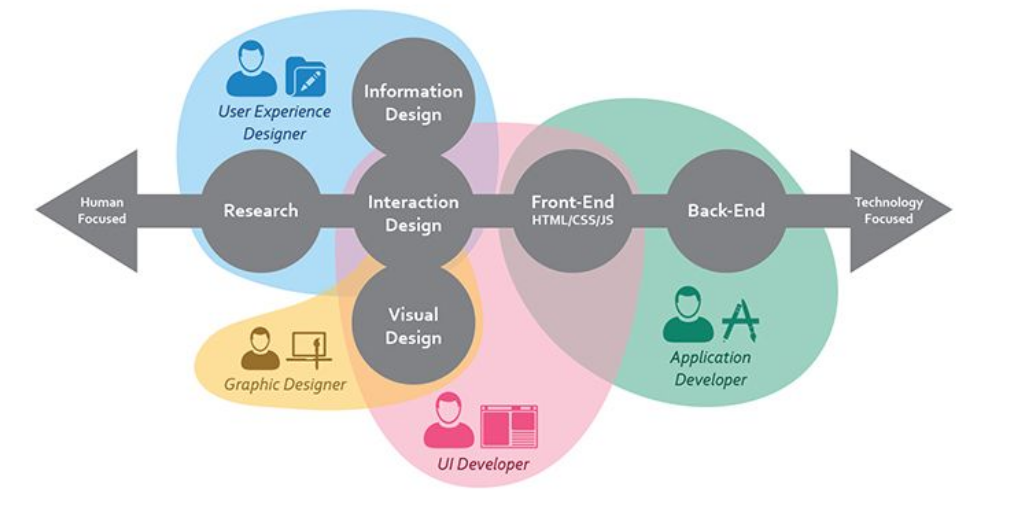
\includegraphics[scale = 0.4]{immagini/UX_and_UI.png}
	\caption{Le varie aree del design.}
\end{figure}


\chapter{User Interface}
Quando parliamo di \textbf{User Interface o UI}, in italiano Interfaccia Utente, parliamo dello spazio di un sistema dove avviene l'interazione uomo-macchina: il monitor, il mouse, le casse audio e quant'altro.

L'obiettivo di questa interazione è far sì che l'utente possa controllare e far funzionare la macchina in modo efficace, mentre essa reagisce simultaneamente fornendogli informazioni, tramite \textbf{feedback}, aiutandone il suo processo decisionale.

In generale, l'obiettivo dello UI design è quello di produrre una UI che renda facile, efficiente e divertente l'uso di una macchina o di un programma, in modo da massimizzare la User Experience dell'utente finale.

Il termine \textbf{user-friendly} non può essere omesso in questa trattazione: tra un'app facile e piacevole da utilizzare e una solo facile da usare, l'utente medio preferirà sempre la \textbf{prima}.

Le interfacce sono strutturare in uno o più layers. L' \textbf{HID o Human Interface Device} è la periferica con cui l'utente interagisce con il sistema; come ad esempio mouse, monitor, gamepad, ecc...

Lo \textbf{HMI o Human Machine Interface} è un concetto che astrae dall' HID, con HMI, infatti, ci si riferisce allo strato che separa un essere umano che sta utilizzando una macchina dalla macchina stessa. Un device che implementa un HMI è un HID. Quando la macchina in questione è un computer, HMI diviene \textbf{HCI o Human Computer Interface}.

\section{Diversi tipi di interfacce}
Una persona umana possiede cinque differenti sensi che possono essere \textbf{mappati} in cinque categorie di interfacce possibili, più una categoria introdotta con l'utilizzo di visori e giroscopi:
\begin{itemize}
	\item \textbf{Tactile UI} (touch)
	\item \textbf{Visual UI} (sight)
	\item \textbf{Auditory UI} (sound)
	\item \textbf{Olfactory UI} (smell)
	\item \textbf{Equilibrial UI} (balance)
	\item \textbf{Gustatory UI} (taste)
\end{itemize}
La composizione di più UI prende il nome di \textbf{CUI o Composite User Interface}.
Le più comuni CUI sono le \textbf{GUI o Graphical User Interface}, le quali sono composte da interfacce grafiche e tattili. Se si aggiunge anche il suono diventano \textbf{MUI o Multimedia User Interface}.

\pagebreak

È bene sottolineare che \textbf{aggiungere più interfacce per poter interagire con una macchina utilizzando più sensi non è sempre una buona idea}. Giusto per fare un esempio, si prendano in esame i video di Facebook: i video venivano riprodotti con l'audio attivo, ma gli ingegneri di Facebook si sono accorti che la maggioranza delle persone che visualizzavano i video, mutavano immediatamente il suono per varie ragioni (e.g. privacy o utilizzo di Facebook in momenti non opportuni), quindi hanno ben pensato di far partire la riproduzione automatica dei video con il suono mutato e introducendo i sottotitoli per le parti del video parlate. Questo, oltre ad essere un ottimo esempio di MUI riprogettata in GUI, è anche un esempio di tecnica ideata per gli utenti disabili e riusata per far fruire il prodotto a quelle personas che lo utilizzano in momenti in cui non possono usufruire dell'audio.

\section{Categorizzare le CUI}
Le CUI possono essere categorizzare in tre diverse macrocategorie:

\begin{itemize}
	\item \textbf{Standard}: usano dispositivi standard come tastiere, mouse e monitor
	\item \textbf{Virtual}: \textbf{schermano} il mondo reale e creano un mondo virtuale. Tipicamente utilizzano dei caschi VR.
	\item \textbf{Augmented}: \textbf{non schermano} il mondo reale bensì erogano contenuti non completamente digitali che prendono forma nella realtà esterna che circonda l'utente, \textbf{espandendola} appunto.
\end{itemize}

Quando un'interfaccia utente interagisce con tutti i sensi umani viene chiamata \textbf{Qualia Interface}, secondo la \textbf{teoria Qualia}.

Le CUI possono essere anche \textbf{classificate tramite il numero di sensi} con cui è possibile interagirvi. Ad esempio, lo \textit{Smell-O-Vision} è una CUI standard 3S, cioè a 3 sensi, con display, suono e odori. Se si aggiungesse un quarto senso diventerebbe 4S, si pensi ad esempio alle poltrone dei famosi cinema 4D.

\begin{figure}[!h]
	\centering
	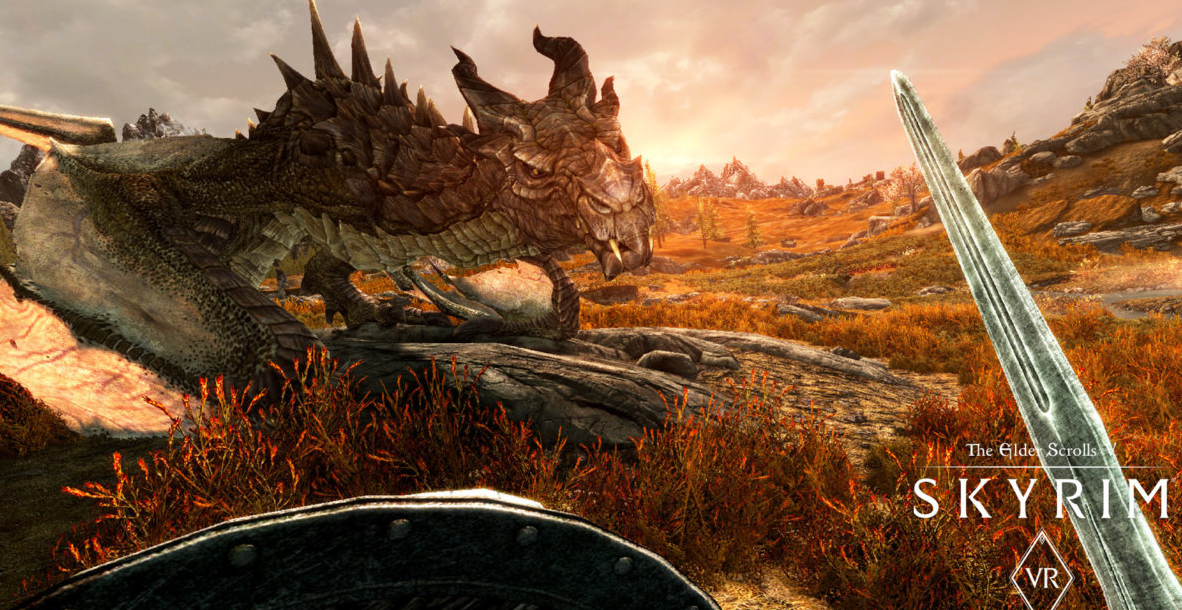
\includegraphics[scale = 0.15]{immagini/SkyrymVR.png}
	\caption{Virtual reality}
\end{figure}\begin{figure}[!h]
	\centering
	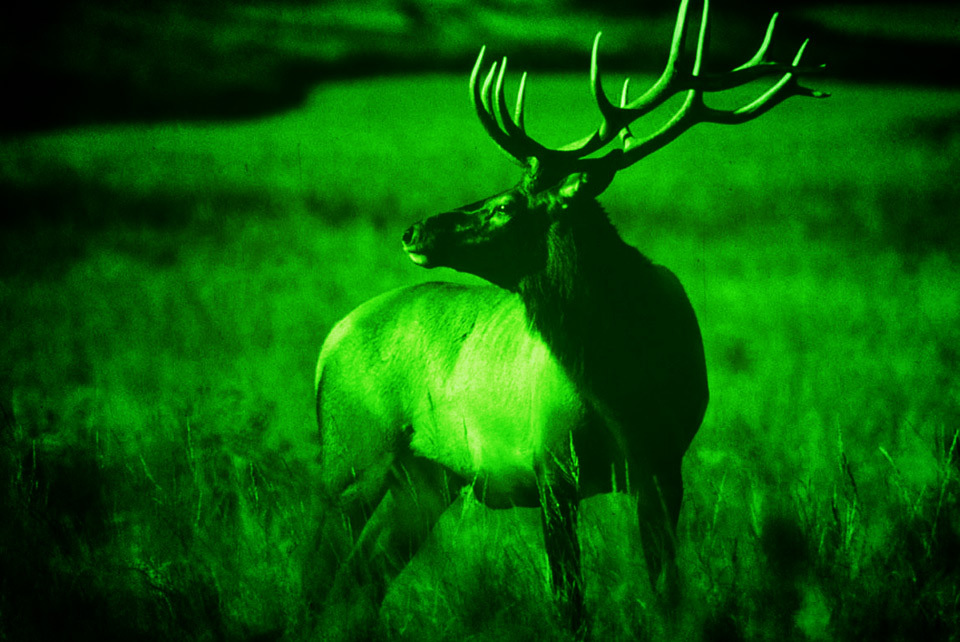
\includegraphics[scale = 0.15]{immagini/Night_vision.jpeg}
	\caption{Augmented reality.}
\end{figure}

\pagebreak


\chapter{Good and Bad Design}
Il buon design valido sempre e per tutti non esiste, poiché si fa design per la user experience di determinate personas. È possibile però individuare due caratteristiche importanti sui cui misurare un buon design:

\begin{itemize}
	\item \textbf{Discoverability}: è la capacità \textbf{innata} di un sistema di veicolare e comunicare i propri possibili usi. Non è detto però che una volta capito cosa si può fare si riesca a farlo. Per avere una buona discoverability si usa tipicamente la \textbf{visibilità}: un rubinetto con i pomelli bene in vista incrementa la discoverability. In un software tale lavoro è svolto dai pulsanti.
	\item \textbf{Understanding}: è la capacità del prodotto di farsi usare correttamente dall'utente.
\end{itemize}

\begin{figure}[!h]
	\centering
	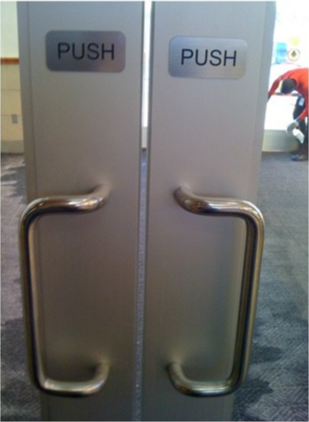
\includegraphics[scale=0.3]{immagini/vis.png}
	\caption{Discoverability and visibility.}
\end{figure}

\begin{figure}[!h]
	\centering
	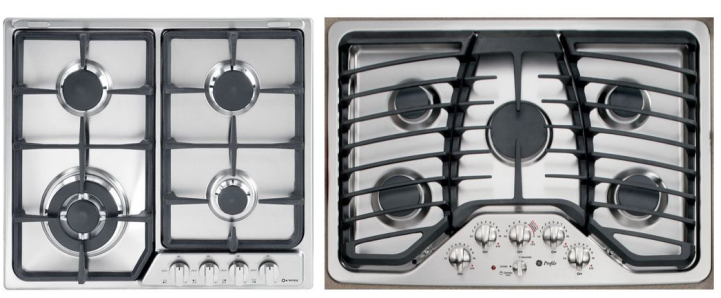
\includegraphics[scale=0.5]{immagini/Fornelli}
	\caption{Understanding.}
\end{figure}

\pagebreak

\section{Design of Useful Things}
\begin{flushleft}
	\textit{Quando le cose vanno bene, si dimenticano subito!}
\end{flushleft}
Questo perché nella psicologia umana \textbf{le cose devono andare bene} per definizione. Quando qualcosa va storto invece, il cervello degli uomini, in particolare l'amigdala, crea un ricordo negativo avente un peso molto maggiore rispetto a un ricordo positivo.

Il design deve quindi preoccuparsi di come funzionano le cose, come vengono controllate e della natura delle interazioni. Quando la progettazione è fatta bene, crea prodotti piacevoli e brillanti, quando è fatta mala, i prodotti sono inutilizzabili e ciò porta a una notevole frustrazione e irritazione da parte dei consumatori.

Le \textbf{macchine} sono concepite, progettate e costruite da esseri umani. Al nostro confronto sono \textbf{assai limitate}: non conservano quella ricca storia di esperienze comuni che ci permette di interagire grazie a un patrimonio collettivo di conoscenze.

Le macchine seguono, di solito, \textbf{regole di comportamento rigide}, piuttosto complicate. Se si sbaglia nel seguirle, anche di poco, la macchina farà comunque quello che le è stato impartito, per quanto insensato e illogico sia. Gli esseri umani sono creativi, dotati di immaginazione e pieni di buon senso, ovvero un abbondante patrimonio di sapere accumulato in anni di esperienza. Le macchine, però, li obbligano ad una grande precisione, cosa a cui non sono avvezzi. Le macchine non hanno nè flessibilità nè buon senso e, spesso, gran parte delle regole seguite da una macchina è nota solo alla macchina stessa e ai suoi progettisti.

Quando non si eseguono queste sue regole segrete e bizzarre, la macchina farà la \textbf{cosa sbagliata} e la colpa verrà scaricata su chi la manovra, accusato di non capirla e di non seguirne i rigidi protocolli. Con gli oggetti di uso comune, il risultato è la frustrazione, con i dispositivi complessi o processi industriali e commerciali, le conseguenze possono essere incidenti anche mortali.

È tempo di \textbf{ribaltare la situazione}, di \textbf{accusare le macchine e la loro progettazione}. La colpa è delle macchine e di chi le ha progettate: sta a loro capire le persone e non il contrario.

Le ragioni della complessità dell'interazione uomo-macchina sono numerose.

Alcune nascono dai limiti della tecnologia attuale, altre da limitazioni intenzionali dei progettisti, spesso per abbassare i costi di produzione. Ma la maggior parte dei problemi deriva dalla totale incomprensione dei principi di design necessari per un'efficiente interazione uomo-macchina. Perché questa deficienza? Perché la progettazione è opera per lo più di ingegneri esperti di ingegneria ma non di psicologia, limitati quindi nella comprensione delle persone.

\textit{"Siamo uomini anche noi"} pensano, \textit{"quindi siamo in grado di capire i nostri simili"}.

I tecnici fanno l'errore di pensare che sia sufficiente la spiegazione logica: \textit{"Basterebbe che leggessero le istruzioni e andrebbe tutto bene"}.

Gli ingegneri sono formati a un tipo di pensiero logico, di conseguenza finiscono per credere che tutti debbano pensare in quel modo e progettano le loro macchine di conseguenza.

È di fondamentale importanza avere ben chiaro il seguente concetto:

\begin{center}
	\textbf{\LARGE Bisogna accettare il comportamento umano per quello che è, non come si vorrebbe che fosse.}
\end{center}

\pagebreak


\chapter{Human Centered Design}
Le persone sono frustate dalla complessità degli oggetti quotidiani. Dalla complessità sempre maggiore del cruscotto dell'auto e dalla crescente automazione della casa, con le sue reti interne. La proliferazione di sistemi complessi per il tempo libero, la comunicazione (e.g. video, audio e giochi elettronici) e le cucine sempre più tecnologiche. La vita di tutti i giorni sembra a volte una battaglia infinita contro la confusione, gli errori continui, la frustrazione e un ciclo interminabile di aggiornamenti e manutenzioni degli apparecchi.

La soluzione è il \textbf{design antropocentrico}, \textbf{human centered desing o HCD}, è una \textbf{metodologia che parte dai bisogni, dalle capacità e dai comportamenti umani, adattando la progettazione a quei bisogni, quelle capacità e quei comportamenti}. Lo HCD è un approccio di design specificamente orientato allo sviluppo di sistemi interattivi, con l'obiettivo di produrre sistemi utili, altamente usabili e che si \textbf{focalizzino sull'utente}.

Il metodo è orientato all'efficienza ed all'efficacia in modo tale da aumentare la soddisfazione dell'utente ed evitare il più possibile gli effetti negativi.

\textbf{Prima l'utente, poi le features!} Lo HCD mette i bisogni, comportamenti e capacità umane prima di tutto e progetta in funzione di esse.

Il problema principale delle UI è la comunicazione, in particolare la comunicazione dalla macchina verso l'uomo, \textbf{una buona interfaccia \textit{sa} comunicare con l'utente}.

Progettare interfacce che funzionano fintanto che le cose vanno bene è relativamente facile, ma \textbf{la comunicazione è ancora più importante quando le cose non vanno bene}. È qui che i progettisti devono concentrare l'attenzione, sui casi in cui le cose vanno storte, non su quelli in cui le cose funzionano secondo i piani. È bene focalizzare l'attenzione soprattutto nel \textbf{comunicare ciò che è andato storto}: bisogna guidare l'utente frustato attraverso la risoluzione del problema poiché, in caso di \textbf{successo}, proverà una \textbf{sensazione positiva}, di affermazione, per aver capito cosa non funzionava e per aver risolto il problema. Ciò crea \textbf{empatia con il sistema}.

\textbf{Evitare quindi la frustrazione e aiutare nella risoluzione quando insorge un problema sono i concetti chiave dello HCD.}
Lo HCD è una filosofia di design che parte dalla \textbf{comprensione delle persone e dei bisogni che esse intendono soddisfare}. Questa comprensione deriva dall'osservazione e dallo studio delle persone che spesso sono inconsapevoli dei loro veri bisogni e magari anche delle difficoltà che incontreranno.

Per capire l'utente bisogna studiarlo ed osservarlo. Tale osservazione non è però sempre possibile, per cui le versioni alfa e beta di un certo sistema non servono solo a fare debugging, ma servono anche per capire che cosa fanno e come si comportano gli utenti: diventa utile avere statistiche sull'utilizzo effettivo del sistema. (e.g. quanti click su un determinato pulsante, quante volte una determinata procedura, ecc...)

\pagebreak

Ottenere \textbf{le specifiche dello HCD} è quindi una delle parti più difficili del design stesso, al punto che il principio è quello \textbf{di evitare di specificare il più al lungo possibile} e procedere con ripetute approssimazioni: si esegue una specifica ad alto livello, se ne implementa una parte, si testa sull'utente finale e tramite il suo feedback, si modifica la parte implementata e la si testa di nuovo. Fatto ciò si passa, magari momentaneamente, ad implementare un'altra parte.

\begin{figure}[!h]
	\centering
	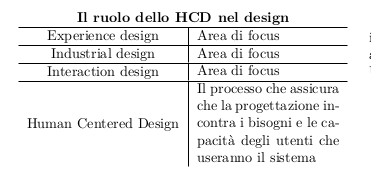
\includegraphics[scale=0.5]{immagini/HCD}
\end{figure}

Si può progettare per il design industriale, per l'interazione e per l'esperienza utente, lo \textbf{HCD non è un'area di focus ma è un metodo}.

\section{Design Thinking vs HCD}
Insieme al termine HCD, spesso si può trovare il termine \textbf{Design Thinking}. I due termini vengono da scuole di pensiero molto valide ma con visioni radicalmente diverse.

Il Design Thinking segue il filone Stanford (dove è nato): è un \textbf{processo di design} con cui progettare nuovi prodotti che verranno poi effettivamente adottati dalle persone. Come processo è più vicino alla \textbf{disruptive innovation} che all'antropocentricità.

Si suddivide in cinque fasi iterative:

\begin{itemize}
	\item \textbf{Empathize}: studiare il pubblico, progettare il prodotto in modo che stabilisca un collegamento empatico con l'utente.
	\item \textbf{Define}: delineare meglio le domande chiave, cioè quali sono i bisogni a cui assolvere.
	\item \textbf{Ideate}: brainstorming, creare soluzioni.
	\item \textbf{Prototype}: costruire una o più idee.
	\item \textbf{Test}: testare le idee e ricevere un feedback.
\end{itemize}

\begin{figure}
	\centering
	\includegraphics[scale=0.5]{"immagini/Fasi Design Thinking"}
	\includegraphics[scale=0.4]{"immagini/Design Thinking vs HCD"}
\end{figure}
Lo HCD è un \textbf{mindset} che viene sovrapposto al Design Thinking: identificato il modello di business, si può applicare lo HCD per assicurare che il prodotto soddisfi \textbf{effettivamente} le esigenze delle persone che lo andranno ad utilizzare.

\pagebreak

\chapter{Principi Fondamentali dell'Interazione}
Un buon design produce un'esperienza piacevole! Ai tecnici non piace molto la parola \textit{esperienza} poiché la considerano troppo soggettiva. Ma se si interrogasse un ingegnere sulla sua automobile preferita descriverà modello e finiture, la sensazione di potenza nell'accelerazione, la maneggevolezza del cambio e dello sterzo.

L'esperienza è cruciale poiché determina \textbf{la tonalità del ricordo} che conserviamo delle interazioni con gli oggetti.

Quando la tecnologia si comporta in maniera inaspettata, gi utenti provano confusione, frustrazione e rabbia: tutte \textbf{emozioni negative}. Se invece comprendono il comportamento della tecnologia, hanno una sensazione di controllo, bravura e persino orgoglio: \textbf{emozioni positive}.

\textbf{Cognizione ed emozione sono profondamente legate}: se non si mette l'utente in un \textit{mood} positivo egli farà più fatica ad usare l'interfaccia. Più l'utente è arrabbiato e frustrato meno è predisposto riutilizzare il prodotto e ad impararne l'uso.

La \textbf{visibilità} o \textbf{discoverability} di un prodotto è il grado di facilità con cui un utente \textbf{scopre cosa fa, come funziona e che tipo di azioni sono possibili}. Tale visibilità è il risultato dell'applicazione di cinque concetti psicologici fondamentali: \textbf{affordance}, \textbf{significante}, \textbf{vincolo}, \textbf{mapping} e \textbf{feedback}. C'è anche un sesto principio, forse il più importante di tutti: \textbf{il modello concettuale del sistema}. Si analizzeranno di seguito:

\section{Affordance}
Il termine affordance, letteralmente \textit{invito}, indica la relazione fra un oggetto fisico e una persona, particolarmente la relazione fra le proprietà dell'oggetto e la capacità dell'utente di determinare in che modo tale oggetto può essere usato.

\textit{Una sedia appare fatta apposta per sostenere qualcosa quindi \textbf{invita} alla seduta. La maggior parte delle sedie è abbastanza leggera da poter essere sollevata e spostata da una singola persona possiamo dire che "
	invita o permette il trasporto, ma alcune sedie sono così pesanti da richiedere l'intervento di più persone. Se però un certo gruppo di individui non ha la forza di sollevare una sedia, per loro la sedia non presenta l'affordance di essere sollevata e trasportata}.

Un'affordance \textbf{non è una proprietà, è una relazione tra un oggetto e una persona}, dipende quindi dalle proprietà sia dell'oggetto che della persona stessa.

Si può anche parlare di \textbf{anti-affordance} nel concetto di \textbf{prevenzione dell'interazione}. Un ottimo esempio sono gli spunzoni per evitare che piccioni o altri tipi di volatili si posino in un cornicione: prevengono l'affordance di sedersi che il cornicione ha verso i piccioni.
Le affordance e le anti-affordance \textbf{devono essere discoverable e perceivable}.

\pagebreak

Questo fatto non è scontato: il vetro, famoso per la sua relativa invisibilità, occulta l'anti-affordance di precludere il passaggio.

Se uno di questi inviti o impedimenti all'uso non è percepibile c'è bisogno di qualche mezzo per segnalarne la presenza: il \textbf{significante}.

\textbf{\underline{N.B.}} È assolutamente sbagliato dire "\textit{metto un affordance}". È corretto dire "\textit{metto un significante}" ma solo se un'affordance è già presente.

\section{Significante}
I progettisti hanno dei problemi pratici: hanno bisogno di sapere come rendere comprensibili gli oggetti che creano. Lavorando sulla grafica degli schermi elettronici, dovevano trovare il modo di indicare quali parti potevano essere sfiorate, battute, fatte scivolare in sù, in giù o di lato, azioni che si potevano eseguire con le dita, con lo stilo o con il mouse.

Un significante è quindi \textbf{un modo per indicare dove effettuare un'azione}, data un'affordance che determina quali azioni sono possibili.

\begin{figure}[!h]
	\centering
	\includegraphics[scale = 0.7]{"immagini/Affordance vs Signifier"}
\end{figure}
\begin{itemize}
	\item \textbf{Affordance}: \textit{cosa si può fare?} \textit{quale azione è possibile compiere?}
	\item \textbf{Signifier}: \textit{dove è possibile fare l'azione?}
\end{itemize}
Molto spesso i significanti \textbf{sono indispensabili} poiché la maggior parte delle affordance sono invisibili. Per fare un esempio basti pensare alle porte scorrevoli: se i cardini non sono visibili, quando vede la maniglia la prima azione che una persona tenta di fare è quella di spingere o di tirare la porta, ma essa non si muoverà, è quindi necessario mettere un significante (e.g. un cartello o una scritta) che indica quale azione è necessaria per aprire la porta.

I significanti posso essere:
\begin{itemize}
	\item \textbf{Voluti o intenzionali}: come un'etichetta, una stringa o un'icona.
	\item \textbf{Accidentali o non intenzionali}: come ad esempio un sentiero tracciato da persone che camminano attraverso un campo o delle persone in fila alla stazione.
\end{itemize}
Nel design \textbf{i significanti sono molto più importanti delle affordances}, perchè comunicano come usare il prodotto o l'interfaccia. Ma come si può associare l'affordance e il significante ad azioni reali? Nella maggior parte dei casi tramite \textbf{convenzioni}. La comprensione di un'affordance percepita è dovuta anche alle convenzioni culturali.

\pagebreak

\begin{figure}[!h]
	\centering
	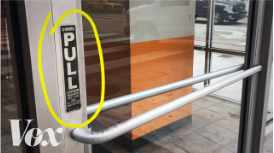
\includegraphics[scale = 0.7]{immagini/sign.png}
	\caption{La scritta pull è un significante, data l'affordance della porta di essere spinta o tirata.}
\end{figure}
\begin{figure}[!h]
	\centering
	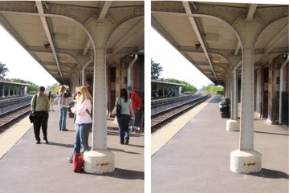
\includegraphics[scale = 0.7]{immagini/sign1.png}
	\caption{Le persone che aspettano il treno sono un esempio di significante sociale.}
\end{figure}

\section{Mapping}
\textbf{Mapping} è un termine tecnico, ripreso dalla matematica, che indica la relazione fra gli elementi di due insiemi.

Il concetto di \textbf{mapping} è di grande importanza nella progettazione di interfacce, in particolare nel \textbf{posizionamento dei significanti}. La disposizione dei significanti può comunicare di più circa l'interfaccia e circa le sue funzionalità. Infatti se si sfrutta una corrispondenza spaziale fra la collocazione dei comandi e quella dei dispositivi comandati, risulta molto più facile capire come usarli.

Il modo migliore per \textit{fare} mapping è quello \textbf{naturale}, perché è un'attività in cui il cervello umano è molto bravo, i bambini imparano a fare mapping fin dai primi anni di vita. È da tenere presente che il concetto di \textbf{naturale} è ben diverso dal concetto di \textbf{universale}, poiché ci possono essere molti mappings che sembrano naturali ma che in realtà sono specifici a una cerchia di culture.

\begin{figure}[!h]
	\centering
	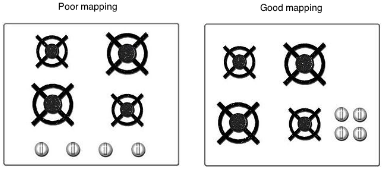
\includegraphics[scale = 0.7]{immagini/mapping.png}
	\caption{Mapping cattivo e mapping buono.}
\end{figure}

\pagebreak

\section{Feedback}
Il feedback è la comunicazione del risultato di un'azione, è una risposta che l'interfaccia dà all'utente.

Il feedback \textbf{deve essere immediato}, anche un ritardo di un decimo di secondo può essere troppo, se il ritardo è troppo lungo l'utente potrebbe rinunciare all'attività che stava compiendo e passare ad altro o addirittura non riuscire a comprendere l'origine del feedback stesso.

\textbf{Deve essere informativo}, non deve portare con sè troppa informazione, ma deve assolvere al proprio obiettivo, deve far capire che un'azione è in corso o che è stato prodotto il risultato che ci si aspetta. Uno scarso feedback può essere peggio di nessun feedback, perché distrae, crea confusione e di conseguenza frustrazione nell'utente.

Un altro caratteristica importante è \textbf{la semplicità}, un feedback non deve essere pedante: troppi annunci o segnali portano le persone ad ignorarli perdendo anche i feedback cruciali e veramente importanti. Il feedback deve essere \textbf{essenziale} e mantenere l'ambiente calmo e tranquillo.

\section{Modello concettuale}
Un modello concettuale è una descrizione altamente semplificata delle funzionalità di un sistema, non deve essere completa o accurata ma \textbf{utile}. I file, le cartelle e le icone che si vedono sullo schermo del computer aiutano le persone a crearsi un modello concettuale dei dati in memoria o delle applicazioni disponibili. In realtà il computer non contiene fascicoli o cartelle: esse sono solo concettualizzazioni ideate per facilitarne l'uso.

\textbf{I modelli semplificati sono preziosi e utili fintanto che le ipotesi che li supportano sono vere.} Nel cloud storage i file sembrano essere sul dispositivo, ma in molti casi il materiale è in realtà nel cloud. Il modello concettuale veicolato è quello di un archivio disponibile sui dispositivi degli utenti. Questo modello semplificato è utile e basta per il normale utilizzo, ma se il collegamento dei servizi si interrompe, può nascere confusione nell'utente: l'informazione è sempre presente sullo schermo, ma egli non può più salvarla o recuperare altri dati, cosa inspiegabile in relazione al modello concettuale precedentemente veicolato.

Il modello concettuale esprime \textbf{come il designer vuole che l'utente percepisca il prodotto}, sarebbe, in un certo senso, l'ambizione di progettare e comprendere la UX. Una volta che i progettisti hanno pensato e progettato il modello concettuale si implementa l'interfaccia, in modo che il modello concettuale venga veicolato all'utente tramite affordances, significanti e mapping presenti su di essa.

Quando una persona interagisce con il sistema o con il prodotto sviluppa un suo modello mentale. Un \textbf{modello mentale} è un modello concettuale nella mente dell'utente che rappresenta il modo in cui, secondo lui, funzionano le cose. Non solo persone diverse possono avere modelli mentali diversi dello stesso oggetto, ma la stessa persona può avere molteplici modelli, pertinenti ciascuno ad un aspetto diverso del suo funzionamento, e persino contraddittori gli uni con gli altri.

\textbf{Più è grande la differenza tra il modello mentale e quello concettuale, più l'utente farà fatica ad usare il sistema.}

L'ideale è che l'utente apprenda un modello concettuale giusto \textbf{direttamente dal device che utilizza}, senza andare a leggere manuali o istruzioni o, peggio ancora, che gli venga trasmesso da terzi. La comprensione di un dispositivo tramite passaparola porta all'\textbf{effetto del telefono senza fili}: l'interpretazione cambia da persona a persona. Per questo vi è necessità che il modello concettuale trasmesso dal prodotto sia pressoché unico in relazione a quello mentale che l'utente si costruisce. In questo contesto vale l'affermazione \textit{less is more} secondo cui se una feature è difficile da veicolare allora è meglio non implementarla.

\pagebreak

\section{Immagine di Sistema}
Le persone si creano di continuo, attraverso l'esperienza, l'addestramento e l'istruzione, modelli mentali di sé, degli altri, dell'ambiente e degli oggetti con cui esse interagiscono.

Questi modelli servono agli uomini da guida per realizzare i loro scopi e comprendere il mondo in cui vivono.

Come fanno gli uomini a formarsi un modello concettuale adeguato dei dispositivi che utilizzano? Non potendo parlare con il progettista, essi si basano su tutta l'informazione accessibile: l'aspetto dell'apparecchio, cosa hanno imparato dall'uso di oggetti simili in passato, cosa comunicano le pubblicità, i venditori, i pieghevoli illustrativi, il sito web e il libretto di istruzioni.

\textbf{L'insieme di tutta questa informazione è l'immagine di sistema}.

\begin{figure}[!h]
	\centering
	\includegraphics[scale = 0.75]{"immagini/Immagine di Sistema"}
\end{figure}

Come illustrato nella figura, il progettista e l'utilizzatore finale del prodotto costituiscono i vertici scollegati di un triangolo. Il vertice del triangolo più a destra è occupato dal modello concettuale del progettista, \textbf{cioè dalla sua concezione del prodotto in questione}.

Una volta commercializzato, il prodotto si stacca dal progettista: lo vediamo infatti isolato nel secondo vertice del triangolo.

\textbf{L'immagine di sistema è tutto ciò che si percepisce dalla struttura fisica prodotta, completa di documentazione, istruzioni,significanti e ogni informazione accessibile dal sito web o dal servizio di assistenza clienti}.

Il modello concettuale dell'utente deriva dall'immagine di sistema, mediante l'interazione con il prodotto, mediante letture, ricerche online e manuali. Il progettista si aspetta che il modello concettuale dell'utente coincida col suo, ma, non essendoci comunicazione diretta fra lui e l'utente, tutto il peso della comunicazione grava invece sull'immagine di sistema.

Questo spiega perché la comunicazione è un aspetto importante del buon design. \textbf{ Per quanto sia geniale il prodotto, se la gente non riesce ad usarlo l'accoglienza sarà cattiva}. Tocca al progettista fornire le informazioni adeguate per rendere il prodotto comprensibile ed usabile. Quel che più conta è presentare un modello concettuale capace di guidare l'utente quando le cose non vanno come dovrebbero.

Un buon modello concettuale è la chiave per avere prodotti comprensibili, di facile uso e gradevoli, e una buona comunicazione è importantissima per ottenere buoni modelli concettuali.

\pagebreak


\chapter{Constraints, Discoverability e Feedback}
\begin{flushleft}
	\textit{In che modo si riesce a capire una cosa che non abbiamo mai visto prima?}
\end{flushleft}

Non c'è altro da fare che combinare l'informazione presente nel mondo esterno con quella che si ha in testa.

L'insieme di conoscenze che si trovano nel mondo comprende le affordances, i significanti visibili, le corrispondenze fra quelle parti degli oggetti che sembrano comandi o punti da manipolare, le azioni risultanti e i vincoli fisici che limitano ciò che è possibile fare.

La conoscenza si ha in mente comprende i modelli concettuali, i vincoli culturali, semantici e logici del comportamento, le analogie fra la situazione attuale ed esperienze precedenti.

\begin{figure}[!h]
	\centering
	\includegraphics[scale = 0.7]{"immagini/Modellino Lego"}
	\caption{Un modellino lego.}
\end{figure}

Si prenda come esempio il modellino Lego presente in figura: ha 15 pezzi, solo alcuni specializzati, molti altri sono di grandezza e forma uguale ma di colori diversi. Combinando i vincoli fisici con quelli culturali, semantici e logici si riesce a costruire il modellino senza istruzioni, mettendo ogni pezzo nella sua giusta posizione.

Vincoli fisici limitano le parti che possono andare insieme, i vincoli culturali e semantici impongono restrizioni precise a tutti i pezzi restanti e se rimane fuori qualche pezzo l'incastro è dettato dalla logica.

\textbf{I vincoli sono indizi potenti}, che limitano l'insieme delle azioni possibili. L'uso intelligente dei vincoli in sede di design permette alle persone di decidere prontamente il giusto corso d'azione, anche in una situazione del tutto nuova.

\pagebreak

È possibile categorizzare i vincoli in \textbf{quattro} classi:
\begin{itemize}
	\item \textbf{Vincoli fisici}: si affidano a proprietà del mondo fisico, senza alcun bisogno di istruzioni o di addestramento. Nell'esempio della motocicletta Lego ritroviamo questo vincolo nei pezzi che si incastrano solo in un determinato verso.
	\item \textbf{Vincoli culturali}: si affidano alle abitudini culturali, sociali, comportamentali che possono cambiare nel tempo. Con \textbf{vincolo culturale} s'intendono anche le convenzioni. Nell'esempio della motocicletta Lego ritroviamo questo vincolo nel saper determinare la collocazione delle luci: bianco all'anteriore e rosso al posteriore.
	\item \textbf{Vincoli semantici}: si affidano al significato della situazione per circoscrivere l'insieme delle azioni possibili, si basano sulla conoscenza della situazione e del mondo. Nel caso della motocicletta, c'è un'unica collocazione sensata per il motociclista, deve stare seduto guardando in avanti.
	\item \textbf{Vincoli logici}: dettati dalla semplice e pura logica umana. Se avanzasse un un solo pezzo per assemblare la motocicletta, grazie alla logica sapremo dove collocarlo nella sua giusta posizione.
\end{itemize}

Un buon designer può sfruttare questi vincoli per veicolare l'utente verso un modello mentale del prodotto che si avvicini il più possibile al modello concettuale desiderato ed in tal modo garantirgli una UX gradevole.

\section{Vincoli e mapping}
Vincoli e mapping a volte si confondono tra di loro. Una serie di interruttori mappati in maniera opportuna infondono un vincolo logico che permette all'utente di non sbagliare, si intuisce perfettamente cosa verrà azionato da quell'interruttore posto in quel determinato punto. \textbf{Mapping forti possono diventare dei vincoli logici}.
L'assenza di vincoli e mapping genera, come già ribadito più volte, frustrazione poiché crea una interfaccia poco chiara e difficile da comprendere.
\begin{figure}[!h]
	\centering
	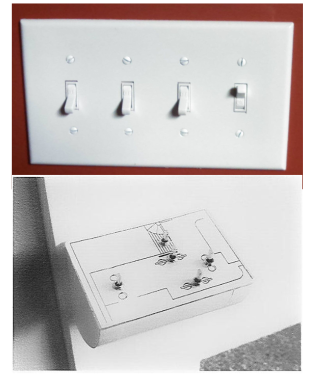
\includegraphics[scale=0.67]{immagini/Interruttori}
	\caption{Un interruttore per le luci di una stanza che imita la piantina del locale.}
\end{figure}

\pagebreak

\section{Funzioni Obbliganti}
\textbf{Le funzioni obbliganti sono una forma di vincolo fisico}: consistono di situazioni in cui le azioni sono vincolate in modo che un passaggio mancato impedisca di procedere al successivo.

Sono il caso estremo di vincoli atti ad impedire un comportamento inappropriato.

Non tutte le situazioni permettono l'uso di vincoli così forti, ma il principio generale è applicabile negli ambiti più diversi.

Si esaminano ora tre di questi metodi:
\begin{itemize}
	\item \textbf{Interlock}: obbliga a eseguire le operazioni nella sequenza dovuta. Usati soprattutto nell'ambito della sicurezza. \textbf{Per compiere un task si deve eseguire una serie di passi.}
	\item \textbf{Lock-in}: mantiene attiva una funzione impedendo che qualcuno la interrompa prematuramente. È usato molto in ambito informatico (e.g. ogni tentativo di uscita da un'applicazione senza salvare è prevenuto da un messaggio di allerta che chiede la conferma dell'intenzione). \textbf{Per finire un task si deve compiere un'azione.}
	\item \textbf{Lockout}: impedisce l'ingresso in uno spazio pericoloso o impedisce che succeda qualcosa. Può essere considerato l'opposto del lock-in. Un esempio di stampo informatico, sono gli \textbf{alert VM 18} che si possono trovare su alcuni siti. \textbf{Per iniziare un task si deve compiere un'azione.}
\end{itemize}

\begin{figure}[!h]
	\centering
	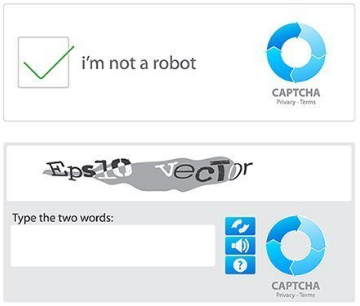
\includegraphics[scale=0.4]{immagini/cap.png}
	\caption{I captcha sono un esempio di interlocks.}
\end{figure}

\section{Activity-Centered Control}
Il mapping spaziale dei comandi non sempre è il più opportuno.

In molti casi è meglio avere interruttori diversi per attività diverse: \textbf{comandi centrati sulle attività}.

Azionando un semplice comando si impostano una serie di oggetti per svolgere una determinata attività, senza comandarli uno ad uno. In molti auditorium ci sono interruttori con indicazioni \textit{video}, \textit{computer}, \textit{piena luce} e \textit{lezione} che impostano il microfono, le luci della sala, il proiettore e quant'altro.

Questo schema è eccellente in teoria, ma nella pratica è difficile da realizzare bene, soprattutto è necessario valutare gli \textbf{imprevisti} e le possibili risoluzioni.

Per carità, il metodo è giusto, purché la gamma di attività sia scelta in modo da corrispondere alle situazioni reali. Ma anche in quel caso saranno pur necessari dei comandi manuali, perché si presenteranno sempre esigenze inattese, che richiederanno una regolazione particolare dei dispositivi.


\chapter{How do people do things}
\begin{flushleft}
	\textit{
		È facile imparare alcune azioni elementari per far funzionare un dispositivo tecnico. Ma cosa succede se le cose non vanno come dovrebbero? Come può l'utente accorgersene, e scoprire cosa fare? }
\end{flushleft}

Per chiarire meglio tutto questo è bene soffermarsi prima sulla psicologia umana e sui modi con cui gli uomini scelgono e valutano le proprie azioni. Fatto ciò si passerà a esaminare il ruolo della cognizione e delle emozioni in tale processo: il piacere quando le cose funzionano senza intoppi e la frustrazione quando le aspettative iniziali degli utenti non sono realizzate.

\section{I Golfi dell'Esecuzione e della Valutazione}
Quando usiamo un oggetto, ci si trova davanti due golfi: il \textbf{golfo dell'esecuzione}, nel quale si cerca di indovinare cosa fare, e il \textbf{golfo della valutazione}, in cui ci si sforza di capire cosa è successo. Il compito del progettista è quello di aiutare gli utenti a superare i due golfi e renderli il meno profondi possibili.

\begin{figure}[!h]
	\centering
	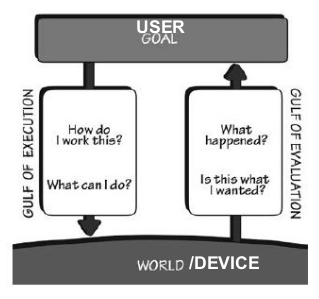
\includegraphics[scale=0.73]{immagini/Golfi}
	\caption{Golfo dell'esecuzione e golfo della valutazione.}
\end{figure}

Il \textbf{golfo della valutazione} corrisponde allo sforzo necessario per interpretare lo stato fisico del dispositivo e capire fino a che punto sono state realizzate le aspettative e le intenzioni iniziali. Il Golfo è stretto quando il dispositivo fornisce informazioni sul proprio stato, in una forma facile da cogliere e interpretare.

\pagebreak

\begin{flushleft}
	\textit{
		Quali sono gli elementi progettuali più importanti per superare il golfo della valutazione?}
\end{flushleft}

Il \textbf{feedback} e un \textbf{modello concettuale adeguato}.

\begin{flushleft}
	\textit{Quali sono gli elementi progettuali più importanti per superare il golfo dell'esecuzione?}
\end{flushleft}
\textbf{Significanti}, \textbf{constraints}, \textbf{buon mapping} e un modello concettuale adeguato.

Entrambi i golfi sono presenti in molti apparati. Si incontrano spesso difficoltà, puntualmente liquidate accusando sè stessi. Di fronte alle difficoltà nell'uso di congegni che ci si aspetta di saper usare si finisce inevitabilmente col pensare di essere stupidi. Oppure, con dispositivi dall'aspetto più complicato, semplicemente ci si arrende, pensando di essere incapaci di utilizzarli. Queste spiegazioni sono entrambe sbagliate. \textbf{Le difficoltà hanno origine nel design, non nell'utente}.

\section{I sette stadi dell'azione}
Compiere un'azione implica due fasi: \textbf{esecuzione e valutazione degli effetti}, \textbf{fare e interpretare}. Sia l'esecuzione che la valutazione richiedono che si capisca come funziona l'oggetto su cui si applica l'azione e quali risultati essa produce. Entrambe le fasi influiscono sullo stato emotivo dell'utente.

Un progettista deve conciliare il compito che l'utente vorrebbe eseguire e tutte le possibili azioni fisiche che può compiere per eseguirlo. Una volta che l'utente specifica quali azioni compiere, bisogna far in modo le esegua concretamente: ciò costituisce lo \textbf{stadio dell'esecuzione}. \textbf{Identificato il goal, o scopo, l'utente discende attraverso i tre stadi dell'esecuzione: pianificare, specificare ed eseguire.}

\textbf{La valutazione si articola anch'essa in tre stadi: percepire, interpretazione, confrontare.}

Ecco così che si hanno i \textbf{sette stadi dell'azione}: uno per lo scopo, tre per l'esecuzione e tre per la valutazione.
\begin{itemize}
	\item \textbf{Scopo}: definire l'obiettivo.
	\item \textbf{Progettare}: definire l'azione da eseguire.
	\item \textbf{Specificare}: costruire una sequenza d'azione.
	\item \textbf{Eseguire}: eseguire la sequenza specificata.
	\item \textbf{Percepire}: osservare lo stato del mondo.
	\item \textbf{Interpretare}: elaborare la percezione.
	\item \textbf{Confrontare}: rapportare il risultato allo scopo.
\end{itemize}
\begin{center}
	\includegraphics[width=0.5\linewidth]{"immagini/Sette stadi"}
\end{center}
La maggior parte delle azioni non richiede che si percorrano tutti i sette stadi in sequenza, ma quasi nessuna attività si risolve in tramite un'azione singola.

Di solito si applicano numerose sequenze e l'intera attività può durare ore o giorni. Ci sono molteplici circuiti di feedback, con cui i risultati di un'attività vengono usati per indirizzare l'utente verso altre, in cui uno scopo genera scopi accessori e ogni un progetto sotto-progetti. Ci sono attività in cui lo scopo originario è addirittura dimenticato, scartato o riformulato.

I sette stadi offrono uno schema per sviluppare nuovi prodotti o servizi. I golfi dell'esecuzione e della valutazione sono i punti più ovvi da cui partire, offrendo entrambi spunti per migliorare il prodotto. I progettisti devono svilupparne capacità di osservazione.

\section{Tre livelli di Processing}
Gli stadi dell'azione possono essere associati a tre livelli di processing mentale: viscerale, comportamentale e riflessivo.

\begin{itemize}
	\item \textbf{Livello viscerale}: è il livello più elementare, permette di rispondere prontamente in maniera subconscia, senza consapevolezza o controllo cosciente.
	\item \textbf{Livello comportamentale}: è la sede delle abilità apprese durante circostanze più o meno simili a quelle attuali. Durante l'esecuzione, il livello comportamentale è guidato dalle aspettative, e durante l'attesa di conferma di tali aspettative è invece guidato dalle emozioni. Il livello comportamentale stabilisce in che modo si compie una determinata azione e in che modo si interpreta un determinato feedback.
	\item \textbf{Livello riflessivo}: è il livello della cognizione conscia, è qui che si sviluppa la comprensione profonda e hanno luogo il ragionamento e i processi decisionali. Qui fanno capo i livelli più alti di emotività: soddisfazione e orgoglio, ma anche frustrazione e senso di colpa.
\end{itemize}

\begin{figure}[!h]
	\centering
	\includegraphics[scale=1]{"immagini/Livelli di Processing"}
\end{figure}

\pagebreak

\textbf{Veicolare informazioni all'utente mentre egli si trova nel livello riflessivo è estremamente efficace}. Al livello riflessivo il suo pensiero è conscio e le emozioni che egli produce sono le più durature.

Gli stimoli riflessivi sono parte integrante del ricordo degli eventi, è importante quindi creare nell'utente ricordi positivi mentre egli è in questo stadio dell'azione, perché tali ricordi sono i più duraturi.

Inoltre è la riflessione, intesa come pensiero cosciente, che induce a consigliare un prodotto e raccomandarne l'uso o magari a sconsigliarlo.

I tre livelli di elaborazione contribuiscono tutti insieme a determinare lo stato emotivo e cognitivo dell'utente. Funzioni riflessive di alto livello possono mettere in moto emozioni più elementari e  queste, a loro volta, possono stimolare attività cognitive di tipo riflessivo.

\section{I sette Principi Fondamentali della Progettazione}
Il modello a sette stadi del ciclo d'azione è un prezioso sussidio per il design, in quanto introduce una lista di domande fondamentali. In generale, ogni stadio dell'azione richiede specifiche strategie progettuali, e, viceversa, presenta occasioni proprie di disastro.

Ne derivano dunque sette domande, a cui dovrebbe poter rispondere chiunque stia usando un determinato prodotto.

\begin{itemize}
	\item \textbf{Cosa voglio ottenere?}
	\item \textbf{Quali sono le sequenze d'azione alternative?}
	\item \textbf{Quale azione posso fare ora?}
	\item \textbf{Come faccio questa azione?}
	\item \textbf{Cosa è successo?}
	\item \textbf{Cosa significa?}
	\item \textbf{Va bene? Ho realizzato il mio scopo?}
\end{itemize}

\begin{figure}[!h]
	\centering
	\includegraphics[scale=0.55]{"immagini/Sette Domande"}
\end{figure}

\pagebreak

Il progettista ha la responsabilità di garantire che a ogni stadio dell'azione il prodotto fornisca l'informazione necessaria per proseguire correttamente.

L'informazione che serve a rispondere alle domande nelle fasi attuative è definita come \textbf{feedforward}.

L'informazione che aiuta a capire quello che è successo nella fasi percettive è definita invece come \textbf{feedback}.

Il \textbf{feedforward} si realizza mediante l'uso opportuno di significanti, vincoli e mapping, anche il modello concettuale ha un ruolo importante.

Il \textbf{feedback} è dato dall'immediato cambiamento di stato che il prodotto deve mostrare all'utente e, anche qui, una parte importante è svolta dal modello concettuale.

Sia il \textbf{feedback}, che il \textbf{feedforward} devono presentarsi in una forma facilmente interpretabile da chi utilizza il sistema. La presentazione deve corrispondere alla visione che le persone hanno dello scopo che vogliono realizzare e alle loro aspettative. L'informazione erogata deve essere immediatamente comprensibile.

Dalle risposte relative ai sette stadi dell'azione si ricavano sette principi fondamentali del design:

\begin{itemize}
	\item \textbf{Visibilità}: è bene che sia facile scoprire immediatamente quali azioni sono possibili e qual è lo stato attuale del dispositivo.
	\item \textbf{Feedback}: è opportuno che ci sia un'informazione completa e continua riguardo ai risultati delle azioni e allo stato attuale del prodotto o del servizio. Dopo aver eseguito un'azione, deve essere facile determinare il risultato.
	\item \textbf{Modello Concettuale}: il design dovrebbe fornire tutta l'informazione necessaria per creare un buon modello concettuale del sistema, che favorisca la comprensione e la sensazione di controllo da parte dell'utente. Il modello concettuale potenzia sia la visibilità, sia la valutazione dei risultati.
	\item \textbf{Affordance}: è bene che le affordance siano fatte apposta per rendere possibili le azioni desiderate e impossibili quelle indesiderate.
	\item \textbf{Significanti}: un uso efficace dei significanti assicura la visibilità e la comprensibilità dei comandi.
	\item \textbf{Mapping}: è necessario che la relazione fra i comandi e le rispettive azioni obbedisca ai principi del buon mapping, sostenuto, per quanto possibile, dalla disposizione spaziale e dalla contiguità temporale.
	\item \textbf{Vincoli}: bisogna fornire vincoli fisici, logici, semantici e culturali, in modo tale da guidare l'azione e facilitandone l'interpretazione.
\end{itemize}
Questi sette principi sono mappati uno ad uno sugli stadi d'azione dell'utente.

È bene concludere con una nota la parte dedicata a strumenti, metodi ed elementi per il design dello human-computer interaction: per molte attività quotidiane , gli obiettivi e le interazioni non sono ben definiti, \textbf{sono più di tipo opportunistico che frutto di una pianificazione}.

Le azioni opportunistiche sono quelle in cui il comportamento scaturito dalle circostanze prevale sulla pianificazione. Gli utenti in questi casi agiscono in maniera non controllata e quindi non prevedibile.

È difficile fare buon design per queste situazioni, anche attenendosi a tutti i principi esposti fino ad ora: l'utente che agisce in maniera opportunistica romperà in ogni caso questi schemi.

\pagebreak

\section{Disruptive Innovation}
\begin{flushleft}
	\textit{“People don’t want to buy a quarter-inch drill. They want a quarter-inch hole!”}
\end{flushleft}
La maggior parte dell'innovazione è fatta come miglioramento incrementale di prodotti già esistenti. La \textbf{disruptive innovation} riguarda l'innovazione non lineare, consiste in un completo salto di binario. Vuole introdurre idee radicali che portano a progettare nuove categorie di prodotti nel mercato.

\begin{figure}[!h]
	\centering
	\includegraphics[scale=0.6]{"immagini/Disruptive Innovation"}
\end{figure}

Ciò è effettuato riconsiderando l'obbiettivo tramite un procedimento chiamato \textbf{root cause analysis}, che può essere decomposto in quattro fasi.

La \textbf{root cause analysis} è quindi fatta:

\begin{enumerate}
	\item Descrivendo chiaramente il problema.
	\item Tracciando il flusso degli eventi che ha fatto in modo che da una situazione di normalità emergesse un problema.
	\item Distinguendo le cause principali dalle cause secondarie.
	\item Tracciando un grafico che descrive le relazioni tra le cause principali e il problema.
\end{enumerate}

\section{Agile}
\begin{flushleft}
	\textit{Si supponga che la progettazione non sia un problema e che si possegga l'analisi completa di un un processo, come fare ad innovare?}
\end{flushleft}
L'\textbf{Agile} è un \textbf{modo di pensare} che rientra nella categoria del \textbf{Design Thinking}.
È un \textbf{metodo di lavoro}: il Design Thinking è un modo di porsi nella soluzione dei problemi, mentre invece l'\textbf{Agile} è il modo in cui si applicano i metodi del Design Thinking per sviluppare software, il primo infatti
porta a identificare una soluzione, l'\textbf{Agile invece è un metodo strutturato per lo sviluppo di software}.
Nell'\textbf{Agile} il focus è posto sugli individui e l'interazione con essi piuttosto che sui processi e sui tools. Il risultato è un software che funziona invece che grandi  e verbosissime documentazioni. Uno dei punti fondamentali è lo sviluppare capacità di adattamento al cambiamento.
Le regole non sono dettate dai programmatori o da un capo che prende le decisioni,
tutto è guidato dal processo di design. Il grande punto di forza dell'Agile rimane comunque quello dell'\textbf{adattabilità}. La mancanza di struttura o documenti non è anarchia, anzi è fulcro di grande collaborazione e sintonia tra il team.

\pagebreak

\chapter{Design Phases}
\begin{flushleft}
	\textit{Quali processi e metodi utilizzare per portare avanti il progetto di un
		prodotto software?}
\end{flushleft}

In questo capitolo si analizzeranno diversi processi.
Essi non vanno identificati come fasi ben definite e statiche, da seguirsi una dietro l'altra, bensì come \textbf{fasi} \textbf{dinamiche} e \textbf{alternabili}.

\section{Personas}
Identificato correttamente il problema mediante la \textbf{Task Analysis}, come si  possono creare elementi individuali? Come si identificano le così dette le \textbf{Personas}?

\begin{figure}[!h]
	\centering
	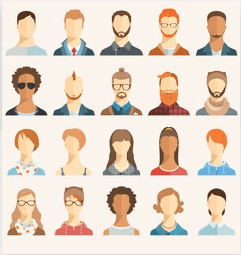
\includegraphics[scale=0.55]{immagini/Personas.png}
\end{figure}

Il primo passo da fare dopo la Task Analysys è \textbf{identificare le personas}.
Una \textbf{personas} è l'\textbf{archetipo di uno dei possibili utenti}. Scrivere e
identificare le personas aiuta a colmare la distanza tra il cliente e l'azienda, in modo da capire cosa vuole e cosa si aspetta l'utente dal prodotto, ma anche cosa gli crea frustrazione nell'usarlo. Esistono molte \textbf{tecniche} atte a fare fare un'analisi degli utenti e che aiutano i progettisti a identificare e a scrivere le personas:

\begin{itemize}
	\item \textbf{Task Analysis}.
	\item \textbf{Feedback} tra i quali: analisi delle attività, interviste e focus groups.
	\item \textbf{Prototipazione}.
\end{itemize}

Sorge spontanea la domanda seguente: \textit{ma quante personas è bene definire}?
Per rispondere a questa domanda ci si basa sul \textbf{Principio di Pareto}: \begin{center}
	\textit{Concentrarsi sul 20\% degli utenti che utilizzerà il prodotto per l'80\% dell'uso complessivo.}
\end{center}

\pagebreak

\section{Requirements}

Un \textbf{requirement} è un servizio o una caratteristica che soddisfa un bisogno di un utente.
I requirements possono essere funzioni, vincoli, regole aziendali o altri tipi di elementi di cui il prodotto deve essere dotato per soddisfare le esigenze degli utenti. È quasi ovvio che trovare i \textbf{requirements corretti} risulta molto più \textbf{semplice} se in precedenza sono state \textbf{individuate} e \textbf{descritte} le \textbf{personas}.

Infatti è controproducente scrivere anticipatamente i requirements,
è complesso se non impossibile descriverli tutti all'inizio di una fase di progettazione. Risulta più facile descrivere i requirements con l'avanzamento del progetto, in modo da poter capire come modificare, eliminare o aggiungere i requirements giusti, tenendo in considerazione anche le personas a cui è destinato il prodotto finale.

Il \textbf{requirements driven development} è un approccio complesso e oneroso e va in \textbf{contrasto} con il metodo \textbf{Agile} che richiede si sia sempre pronti al cambiamento. Questo approccio così poco flessibile sta andando sempre meno di moda tuttavia è bene seguirlo una volta definiti i requirements per quel 20\% di software che utilizzerà l'80\% delle personas.

Esistono \textbf{due tipi di requirements} per il mondo della UI:

\begin{itemize}
	\item \textbf{Funzionali}:
	      descrivono quali funzionalità deve avere il software. Rispondono alla domanda:
	      \textit{Cosa fa?}
	\item \textbf{Non funzionali}: specificano i tratti qualitativi del prodotto. Rispondono alla domanda: \textit{Come lo fa?} e descrivono inoltre
	      attributi come sicurezza affidabilità e manutenibilità.
\end{itemize}

\section{User Stories}
Dopo aver definito \textbf{personas} e \textbf{requirements}, il prossimo passo è la scrittura delle \textbf{User Stories}.

Una \textbf{user story} è una breve descrizione che identifica l'utente insieme al suo
obiettivo e alle sue necessità, determina \textbf{chi è}, \textbf{di cosa ha bisogno e perché ne ha bisogno}. Tipicamente ci sono una o più user stories per ogni personas, ma \textbf{non il contrario}: avere più personas per una user story significa aver descritto la medesima persona con termini differenti e quindi averne introdotta una ridondante.
Se una user story non copre tutte le sfaccettature della singola persona che dovrebbe descrivere è indizio del fatto che tale persona potrebbe essere troppo \textbf{ampia}, ed è bene che venga suddivisa in più personas.

Una user story è un \textbf{requirement} espresso \textbf{dalla prospettiva del cliente}.

Con le user stories si ottengono due importanti risultati: si \textbf{migliorano le descrizioni delle personas}, migliorandone il dettaglio e arricchendole con una narrativa, e si ha un elemento tangibile per valutare lo sviluppo del prodotto e fare il punto della situazione.
Esiste uno schema ben preciso per scrivere una user story:

\begin{center}
	\textbf{\large As a [role], I want [feature] because [reason]}
\end{center}

\begin{flushleft}
	\textit{Chi scrive le user stories?}
\end{flushleft}

\textbf{Tutti}! È responsabilità del proprietario del prodotto assicurarsi che vengano scritte delle stories giuste e corrette, ma non significa che le debba
scrivere lui stesso. Nel corso di un buon progetto Agile ci si aspetta che ogni membro del team partecipi alla scrittura delle user stories secondo un \textbf{metodo collaborativo}.

\pagebreak

\begin{flushleft}
	\textit{A che livello è bene scriverle?}
\end{flushleft}

Uno dei grandi benefici delle user stories è che possono essere
scritte a \textbf{vari livelli di dettaglio}.

Possiamo avere user story di livello \textbf{epic}, ovvero in grado di
coprire un grande quantità di funzionalità, tipicamente sono disutili ma possono diventare interessanti se spacchettate in user stories più piccole e, di conseguenza, più dettagliate. Una \textbf{user story epic} può essere \textbf{divisa} in decine o centinaia di user stories più piccole.

I dettagli possono essere aggiunti sostanzialmente in due modi:
\begin{enumerate}
	\item Suddividendo una user story in user stories più piccole e quindi più dettagliate.
	\item Aggiungendo \textbf{condizioni di soddisfacimento dell'utente}, ovvero  dettagli che contribuiscono al grado di soddisfacimento dell'utilizzatore del prodotto, suddividendole per ogni eventuale membro di soddisfacimento. Quest'ultima è una tecnica molto difficile da utilizzare nel mondo della progettazione software.
\end{enumerate}

\section{Scenarios}

Gli \textbf{scenarios} sono l'\textbf{evoluzione delle user stories}. Una user story sintetizza in brevi frasi cosa fa l'utente con il software e quale bisogno deve soddisfare.

Lo \textbf{scenario estende la user story} andando a descrivere anche quali motivazioni hanno portato l'utente ad usare il software e come egli si comporterà nel suo utilizzo. Inoltre gli scopi o \textbf{goals} delle personas vengono \textbf{estesi} e descritti in maniera più ampia.

\begin{flushleft}
	\textit{Ma a cosa serve uno scenario?}
\end{flushleft}

Le \textbf{user stories} sono \textbf{sintetiche}, \textbf{brevi}, dicono cosa sviluppare e poco più, sono informative e comprensibili \textbf{solo} agli \textbf{addetti al mestiere}. Gli \textbf{scenarios}, essendo più ricchi in dettaglio, sono più comprensibili agli \textbf{stakeholders}, quindi sono \textbf{utili per comunicare e interloquire con persone fuori dal team di sviluppo}. Servono soprattutto per allinearsi con le richieste del cliente ma sono  utili anche all'interno del team per allineare le idee.

Un buon scenario risponde alle \textbf{seguenti domande chiave}:

\begin{itemize}
	\item \textbf{Chi è l'utente?}
	\item \textbf{Quale è la motivazione che lo ha spinto ad usare il prodotto e cosa si aspetta da esso?}
	\item \textbf{Qual è il suo obbiettivo?}
\end{itemize}

In alcuni casi uno scenario potrebbe includere anche aspetti circa \textit{come} fare le cose, ma ciò appartiene al mondo degli \textit{use cases} che verranno analizzati successivamente.
Per \textbf{definire gli scenarios}, è necessario \textbf{mapparli}. Bisogna partire \textbf{avendo già definito le personas e le relative user stories}, e individuare per ogni persona un \textbf{key task} che essa deve svolgere. Si possono scrivere gli scenarios racchiudendo una o più
user stories relative alla persona ma tipicamente per ogni persona si descrive  almeno uno scenario. È necessario \textbf{focalizzarsi sul key task} e quindi contestualizzare nel miglior modo possibile il goal dell'utente e come è influenzato dal contesto in cui egli si trova.

Quindi grazie agli scenarios \textbf{possiamo determinare}:

\begin{itemize}
	\item I \textbf{punti più importanti} su cui concentrarsi durante il \textbf{processo di progettazione per l'UX}.
	\item Quali fasi del processo richiedono \textbf{ulteriore revisione e attenzione}.
	\item Le \textbf{principali esigenze e motivazioni dell'utente}.
\end{itemize}

\pagebreak

Ci sono \textbf{tre metodi principali per scrivere gli scenarios}:

\begin{itemize}
	\item Piccoli \textbf{goal or task oriented scenarios}: sono brevi, quasi una semplice estensione della dialettica di una user story.
	\item \textbf{Elaborated Scenarios}: sono versione più elaborata e con molto più contesto.
	\item \textbf{Full Scale Task Scenarios}: sono talmente dettagliati che i singoli task delle attività sono praticamente scritti sotto forma di paragrafo. Sono da evitare poiché si rischia gli scenarios così ottenuti siano uguali agli use cases.
\end{itemize}

\section{Use Cases}

Gli use cases sono la naturale evoluzione degli scenarios.
\textbf{Consistono della completa narrativa di quali azioni l'utente compie per svolgere uno scenario}.

Ogni \textbf{caso d'uso} è una \textbf{serie di step monolitici}, è quindi una nuova task list prodotta dal processo di design per ampliare ulteriormente un concetto analizzato e descritto in precedenza mediante la task analysis.
Uno \textbf{scenario} si concentra su una situazione che coinvolge uno o più \textbf{attori}, mentre un
\textbf{caso d'uso} è incentrato su una \textbf{persona}, come essa si comporta, che decisioni prende e come interagisce con la nostra piattaforma o software. I casi d'uso aggiungono informazione perché aiutano a \textbf{spiegare come dovrebbero comportarsi
	il sistema e il processo}, inoltre aiutano anche nella fase progettuale di brainstorming e danno un'idea su cosa potrebbe andare storto. Forniscono inoltre un elenco di obiettivi che può essere utilizzato per stabilire e valutare la complessità del sistema. I casi d'uso sono \textbf{diretti allo sviluppo}.

Con dei \textbf{casi d'uso ben fatti} si può passare direttamente all'\textbf{implementazione} poiché \textbf{delimitano precisamente cosa deve fare il sistema e come si deve comportare nelle varie situazioni}.

In un caso d'uso sono \textbf{inclusi}:

\begin{multicols}{2}
	\begin{itemize}
		\item \textbf{L'utente}.
		\item \textbf{Cosa vuole fare}.
		\item \textbf{Qual è il suo scopo o goal}.
		\item Gli \textbf{step necessari} per arrivare allo scopo.
		\item I \textbf{feedback} che il sistema restituisce durante i vari step.
	\end{itemize}
\end{multicols}

\textbf{Non sono inclusi} in un caso d'uso:

\begin{multicols}{2}
	\begin{itemize}
		\item Qualsiasi \textbf{dettaglio implementativo o di scelta tecnologica} che non sia un constraint o un requirement.
		\item \textbf{Dettagli} riguardanti l'interfaccia utente.
	\end{itemize}
\end{multicols}

I passaggi da seguire per scrivere un caso d'uso sono:

\begin{multicols}{2}


	\begin{enumerate}
		\item Identificare le \textbf{personas}.
		\item Sceglierne \textbf{una per caso d'uso}.
		\item Identificare i suoi \textbf{obiettivi}.
		\item Discernere i \textbf{task principali} da quelli \textbf{secondari}: applicare il principio di Pareto, quindi focalizzarsi sul basic path e non su casi particolari.
		\item Considerare le sequenze alternative.
		\item Cercare i punti in comune tra i vari casi d'uso e \textbf{accorparli}, riducendoli ove possibile.
		\item Ripetere il procedimento per tutti gli utenti.
	\end{enumerate}
\end{multicols}

Questi passaggi, eseguiti correttamente, consentono di identificare informazioni chiave sugli utenti, utili a costruire prodotti che soddisferanno tutte le possibili personas. \textbf{Ogni passo che ci avvicina all'utente è un passo verso la giusta direzione}.

\pagebreak

\chapter{Human Error}

La maggior parte degli incidenti industriali è causata da errore umano:
le stime si aggirano tra il 75\% e il 95\% del totale.

\begin{flushleft}
	\textit{Come è possibile che tante persone siano così incompetenti?}
\end{flushleft}

La risposta è semplice! Non lo sono, il problema è nella mal progettazione e nel cattivo design.

Si continuano a produrre dispositivi e software che richiedono, a chi li usa, di mantenere per ore un'attenzione ed una vigilanza complete, oppure di memorizzare procedure arcaiche, confuse e usate di rado, magari anche una sola volta nella vita. Si costringono le persone a stare in un ambiente monotono senza nulla da fare per ore e ore, salvo dovere improvvisamente rispondere con rapidità e precisione. Le si sottopone ad un ambiente di lavoro complesso e sovraccarico, dove sono continuamente interrotte durante l'esecuzione di compiti simultanei. L'\textbf{interruzione è una delle cause che più frequentemente portano all'errore umano}.

Uno dei più grandi \textbf{problemi} è l'\textbf{atteggiamento delle persone verso gli errori} commessi. Quando un errore causa perdite economiche o, peggio ancora, danni alle persone, si istituisce una speciale commissione d'inchiesta, che quasi immancabilmente trova i colpevoli.

Il passo successivo è punirli con multe, il licenziamento o addirittura il carcere. Essi vengono incolpati
e puniti o, nella migliore delle ipotesi, incolpati e riaddestrati. Tutto questo però non
risolve il problema: lo \textbf{stesso errore continuerà a presentarsi}.  Per evitare di incorrere nuovamente nell'errore, quando esso viene commesso, è bene  studiarne le cause, per poi ridisegnare il prodotto o le procedure in modo che esso non si ripeta o, se dovesse ripetersi, che i danni siano ridotti al minimo.

\section{Root Cause Analysis}
La \textbf{Root Cause Analysis} consiste nell'indagare l'incidente finché non si trova la singola causa che ne è l'origine. Ovvero il momento nel tempo quando effettivamente qualcuno ha preso decisioni o eseguito azioni sbagliate e,
una volta fatto ciò, accertare da cosa è derivato lo sbaglio. Purtroppo, troppo spesso, il processo si ferma non appena si scopre che una persona ha agito in maniera impropria, additandola come \textit{colpevole}.

Cercare di trovare la causa di un incidente suona bene, ma ha due difetti.

\begin{enumerate}
	\item La maggior parte degli incidenti \textbf{non ha una sola causa}. Da qui il \textbf{modello a groviera degli incidenti} di James Reason.
	\item Solitamente l'analisi delle cause profonde si ferma non appena trovato un errore umano.
\end{enumerate}

\pagebreak

\begin{figure}[!h]
	\centering
	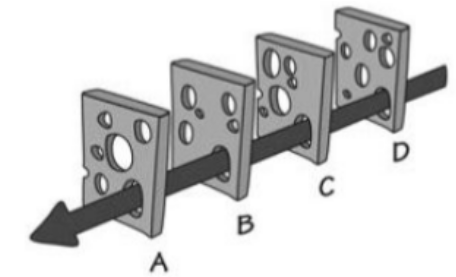
\includegraphics[scale=0.55]{immagini/Groviera.png}
	\caption{Modello a groviera.}
\end{figure}

Se una macchina smette di funzionare per un guasto o un malfunzionamento
si cerca di capire come mai si è rotta o cosa l'ha portata a guastarsi. È
opportuno fare lo stesso quando si scopre un errore umano: \textbf{individuarne le cause}.

Quando durante l'analisi delle cause profonde si incontra, nella concatenazione di cause ed effetti, un errore umano, \textbf{il lavoro è appena cominciato}: bisogna capire \textbf{perché} l'errore \textbf{è accaduto e cosa si può fare per prevenirlo}.

\section{I cinque perchè}

L'analisi delle cause profonde mira a determinare la causa \textbf{prima di un evento}, non la causa immediata.

In Giappone da tempo si usa a questo scopo una procedura detta \textit{"dei \textbf{cinque perché}"} ideata da Sakichi Toyoda e impiegata dalla Toyota nell'ambito del sistema di controllo qualità dei suoi prodotti.

Fondamentalmente quindi quando si cerca la ragione di un evento non ci si deve fermare dopo averne trovata solo una, ma bisogna continuare ad indagare fino a che non si trovano le \textbf{vere cause di fondo}.

Va ripetuta davvero cinque volte?

No, ma chiamarla \textit{procedura dei cinque perché} sottolinea la necessità di proseguire anche dopo aver trovano una causa apparente.

Vediamo un esempio: \textbf{il veicolo non si accende}.

\begin{enumerate}
	\item \textbf{Perché?} La batteria è morta.
	\item \textbf{Perché?} L'alimentatore non funziona.
	\item \textbf{Perché?} La cinghia dell'alternatore non funziona.
	\item \textbf{Perché?} La cinghia dell'alternatore era ben oltre il suo tempo di servizio e non è stata sostituita.
	\item \textbf{Perché?} Il veicolo non è stato mantenuto secondo le tempistiche raccomandate.
\end{enumerate}

Quando le persone sbagliano, bisogna \textbf{cambiare il sistema} in modo da evitare l'errore
e, se non è possibile eliminarlo del tutto, almeno fare in modo di ridurne gli effetti.

Se il sistema lascia sbagliare gli utenti è \textbf{mal progettato}, se il sistema induce all'errore, allora è \textbf{progettato malissimo}.

\pagebreak

\begin{flushleft}
	\textit{Perchè le persone sbagliano?}
\end{flushleft}

Perchè il design si concentra sulle esigenze del sistema
e delle macchine, non su quelle degli utenti. Le macchine hanno bisogno in genere di
comandi precisi, obbligando l'operatore a introdurre esatte informazioni numeriche. Gli esseri umani non sono adatti ad esercitare grande precisione e commettono spesso
errori quando devono digitare lunghe sequenze di numeri o lettere.

Gli umani sono creativi, curiosi, costruttivi, particolarmente bravi nel creare modi nuovi di fare le cose e nel cogliere nuove opportunità. Compiti monotoni, ripetitivi e precisi contraddicono tali qualità e vi entrano in conflitto.

\section{Definizione di errore}
Si definisce \textbf{errore umano} ogni deviazione dal comportamento \textit{appropriato}. Il termine appropriato è da prendere con le pinze, perché in molte circostanze si scopre quale fosse il comportamento giusto solo successivamente.

Generalmente comunque si chiama \textit{errore} ogni comportamento che si discosta da quello generalmente accettato come giusto o adeguato. \textbf{Errore} è il termine generale per tutte le situazioni sbagliate. È possibile dividere gli errori in \textbf{due} classi:

\begin{multicols}{2}
	\centering
	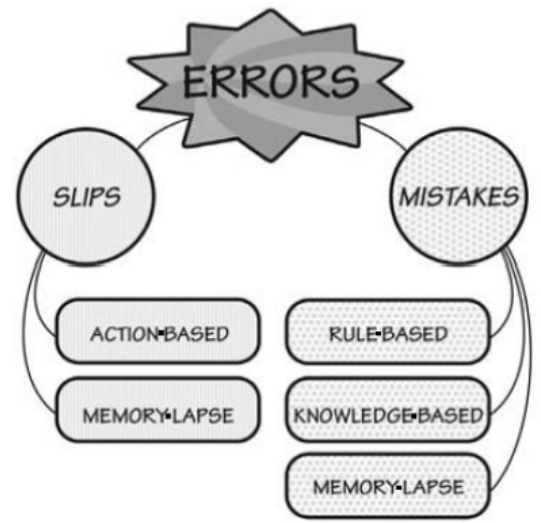
\includegraphics[scale=0.25]{immagini/Errors.png}
	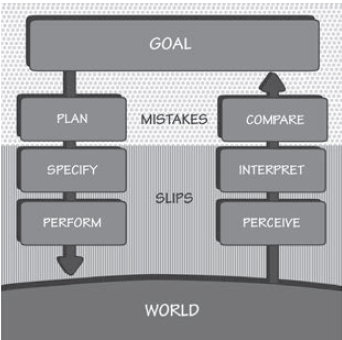
\includegraphics[scale=0.4]{immagini/Errors1.png}
\end{multicols}

\begin{enumerate}
	\item \textbf{Lapsus o Slips}: si ha un lapsus quando s'intende eseguire un'azione e si finisce per eseguirne un'altra. Nel caso del lapsus, l'azione eseguita non è quella voluta. Ci sono \textbf{due tipi principali di lapsus}:
	      \textbf{lapsus di azione e lapsus di memoria}.
	      Nel primo caso si esegue un'azione sbagliata, nel secondo si dimentica di eseguire
	      l'azione o di valutarne i risultati.
	      Esempio di \textbf{lapsus di azione}: versare il latte nel caffè e poi riporre la tazza in frigorifero. L'azione è giusta ma è applicata all'oggetto sbagliato.
	      Esempio di \textbf{lapsus di memoria}: dimenticare di spegnere il fornello dopo aver terminato la cottura. \textbf{I lapsus si hanno nelle fasi attuative e percettive dell'azione.}
	\item \textbf{Errori cognitivi o Mistakes}: si ha un errore cognitivo quando è sbagliato il goal o lo scopo: da quel momento in poi le azioni, anche se eseguite a puntino, fanno parte dell'errore essendo di per sé inappropriate, in quanto parte di un progetto sbagliato. In questo tipo di errore l'azione è corretta ma l'intenzione no.
	      Gli errori cognitivi si suddividono in: \textbf{regola sbagliata}, \textbf{conoscenza sbagliata e dimenticanza}. In un errore generato dall'applicazione della \textbf{regola sbagliata}, la
	      diagnosi della situazione è giusta, ma poi viene scelto un corso d'azione sbagliato,
	      seguendo una regola operativa errata. In un errore causato da \textbf{conoscenza erronea}
	      o \textbf{incompleta}, ad essere sbagliata è la diagnosi stessa della situazione. Gli errori per \textbf{dimenticanza} si hanno invece quando ci si dimentica di qualche passaggio al momento di fissare gli obiettivi, di eseguire una procedura o di valutarne i risultati. \textbf{Gli errori si fanno nelle fasi di tipo cognitivo.}
\end{enumerate}

\pagebreak

\section{Prevenzione dell'errore}

\begin{flushleft}
	\textit{Non dovrebbe essere possibile che un semplice errore provochi un danno diffuso.}
\end{flushleft}

Ecco che cosa dovrebbe essere fatto in fase di prevenzione:

\begin{itemize}
	\item \textbf{Comprendere le cause dell'errore} per minimizzarne il ripresentarsi.
	\item Effettuare \textbf{controlli di sensibilità}, ovvero, chiedersi se le azioni superano il \textit{test del buon senso}.
	\item Rendere possibile \textbf{annullare le azioni} (undo) o rendere più difficile fare ciò che non può essere annullato (per esempio con uso di locks).
	\item \textbf{Rendere} più \textbf{semplice la scoperta e la comprensione degli errori} e semplificarne la risoluzione.
	\item Non trattare l'azione come errore, piuttosto \textbf{aiutare l'utente a compiere correttamente l'azione}.
\end{itemize}

I \textbf{novizi}, gli utenti base, coloro meno esperti del sistema cadono in \textbf{errori per lo più cognitivi} poiché non hanno una base di conoscenza adeguata e sufficientemente strutturata, viceversa, gli \textbf{utenti esperti} che usano il software o il sistema tutti i giorni e che lo conoscono bene commettono più errori di tipo \textbf{lapsus} poiché tendono ad eseguire i compiti in maniera automatica, quasi istintiva, affidandosi al controllo subconscio, mentre un
principiante è costretto a fare molta attenzione, cosicché incorre meno nei lapsus.

Gli \textbf{errori cognitivi} nascono dalla scelta di scopi e piani d'azione inadeguati, oppure, in sede di valutazione, dal confronto errato tra risultati e scopi. In altre parole dipendono da \textbf{informazioni ambigue o poco chiare sullo stato attuale del sistema e dalla mancanza di un buon modello concettuale}.

Si esamineranno adesso quali possono essere le cause di errore e come è possibile prevenirle.

Le \textbf{interruzioni} sono una delle più grandi cause di errore, \textbf{soprattutto i lapsus}. Quando un'attività viene interrotta da qualche evento, il costo in attenzione è molto maggiore della perdita di tempo causata dell'interruzione. Per riprendere il lavoro è necessario ricordare precisamente il precedente stato dell'attività: quale era l'obiettivo, a che punto del ciclo dell'azione si era rimasti e quale era lo stato del sistema.

La maggior parte dei sistemi rende difficile la ripresa di un azione a seguito di un'interruzione. Tuttavia riducendo i passaggi dell'azione è possibile diminuire il costo d'attenzione necessario per riprendere la concentrazione dopo esser stati interrotti.

Un'altra causa di errore sono i \textbf{feedback errati}: avvisi fastidiosi o non necessari che si presentano spesso durante l'uso di un sistema. Spesso vengono silenziati, disattivati o ignorati, \textbf{facendo perdere di significato anche quelli utili per il raggiungimento dello scopo}.

Se si usano i feedback per segnalare errori ed essi sono stati disattivati dall'utente, egli cadrà in errore non conoscendone nemmeno il motivo. \textbf{Avvisi e metodi di sicurezza vanno usati con cura e intelligenza}.

Un numero sempre maggiore di macchine e sistemi offrono informazioni attraverso l'uso di interfacce vocali , ma come tutti gli approcci anche questo ha dei pro e
dei contro. Da una parte consente di fornire informazioni precise, specialmente quando
l'attenzione visiva è diretta da qualche altra parte, ma se l'ambiente è rumoroso o se ci sono diversi avvisi vocali contemporaneamente, tali avvisi possono non essere compresi o risultare addirittura fastidiosi.

\pagebreak

\begin{figure}[!h]
	\centering
	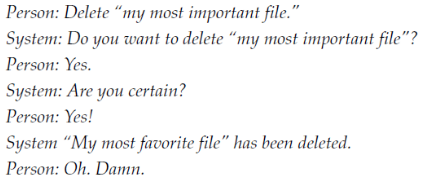
\includegraphics[scale=0.6]{immagini/Damn.png}
\end{figure}

Per prevenire errori è possibile quindi utilizzare:
\begin{itemize}
	\item \textbf{Constraints}: aggiungendo vincoli alle azioni. I sistemi elettronici hanno un'ampia selezione di metodi che possono essere usati per ridurre l'errore. Uno di questi può essere \textbf{segregare i controlli}, cosicché controlli confondibili tra loro vengano piazzati lontani l'uno dall'altro. Un altro è di \textbf{separare i moduli}, cosicché qualsiasi controllo non direttamente rilevante all'operazione corrente non sia visibile a schermo ma richieda uno sforzo extra per essere raggiunto.
	\item \textbf{Undo}: comando che annulla le operazioni effettuate dal precedente. I sistemi migliori hanno \textbf{più livelli di undoing} in modo tale da annullare intere sequenze di azioni.
	\item \textbf{Messaggi d'errore e di conferma}: molti sistemi cercano di prevenire l'errore chiedendo conferma prima di eseguire un comando, specialmente quando l'azione distruggerà qualcosa di importante. Tuttavia queste richieste sono spesso mal temporeggiate, perché \textbf{dopo aver richiesto un'operazione le persone sono solitamente certe di volerla compiere}. Un controllo migliore sarebbe visualizzare sia l'azione da compiere che l'oggetto interessato, con l'opzione annulla o prosegui.\textbf{ I messaggi di avviso sono sorprendentemente inefficaci contro gli errori}.

	\item  \textbf{Controlli di Sensibilità}: i sistemi elettronici presentano il vantaggio di poter controllare che l'operazione richiesta sia \textbf{sensibile} o \textbf{ragionevole}. Ad esempio verificare che l'importo indicato sia giusto, magari esponendo un avviso in caso di numeri eccessivamente grandi.
\end{itemize}

In estrema sintesi e ricollegandosi all'esempio della groviera, per ridurre gli errori si hanno le seguenti possibilità:

\begin{figure}[!h]
	\centering
	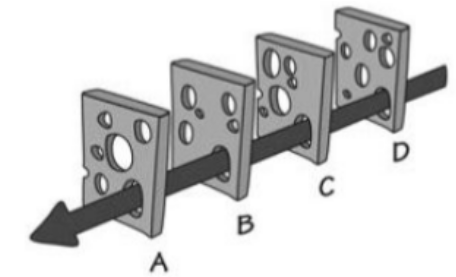
\includegraphics[scale=0.5]{immagini/Groviera.png}
\end{figure}

\begin{itemize}
	\item \textbf{Aumentare il numero di controlli} (le fette).
	\item \textbf{Migliorare il modello concettuale dell'utente}. (ridurre il numero di buchi, o rendere più piccoli i buchi esistenti, magari con un modello concettuale minimale e dei constraints)
	\item \textbf{Allertare l'operatore umano quando diversi buchi si allineano}.
\end{itemize}

\pagebreak

\chapter{Pretotyping}
\begin{figure}[!h]
	\centering
	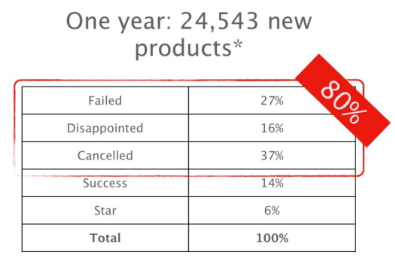
\includegraphics[scale=0.5]{immagini/Fall_mercato.png}
\end{figure}
Un prodotto \textbf{pretotipo} serve a lottare contro la legge di fallimento di mercato. Ogni anno vengono progettati e prodotti quasi 25000 nuovi prodotti l'80\% dei quali non vedrà mai la luce o non arriverà mai nelle case delle persone. Circa il 27\%
falliscono nel percorso di crescita dell'azienda, il 16\% non raggiunge le aspettative degli utenti, trattasi quindi di fallimento di mercato, e per ben il 37\% vengono cancellati durante la fase di lancio.

Del 20\% rimanente, il 14\% sono prodotti che raggiungo il mercato e ci rimangono ma
non hanno successo. \textbf{Solo il 6\% ha veramente successo}. La
\textbf{legge del fallimento di mercato sostiene che la maggior parte dei nuovi prodotti fallirà nel mercato anche se la progettazione e lo sviluppo vengono eseguite in maniera corretta e competente}.
In legge, una persona è considerata innocente fino a prova contraria, mentre nella legge di mercato, \textbf{bisogna considerare ogni prodotto come fallito fino a prova contraria}.

\section{Thoughtland, il mondo dei pensieri}
Quando si progetta un nuovo prodotto, o si ha semplicemente un'idea, ci si trova di fronte a \textbf{due grandi problemi}: il \textbf{lost in translation} e \textbf{il problema della predizione}: il primo sussiste quando l'idea è un'astrazione soggettiva, qualcosa che si può immaginare o visualizzare in testa. Nel momento in cui si prova a comunicarla a qualcun altro però, si incontra un problema
di traduzione, specialmente quando l'idea è nuova ed è diversa da qualsiasi altra cosa
abbia visto l'interlocutore.

Il modo in cui si immagina un nuovo prodotto ed i suoi usi può essere completamente diverso da come gli altri lo immaginano a loro volta. Si può ovviare utilizzando \textbf{termini noti}, infatti, è molto difficile veicolare il modello concettuale all'utente. L'altro problema è conosciuto come il \textbf{problema della predizione}: anche se la comprensione astratta dell'idea che l'interlocutore ha è molto vicina alla propria, egli in quanto essere umano è molto \textbf{scarso per sua natura} nel prevedere se essa potrebbe essere di suo gradimento o meno.

\pagebreak

\section{Thoughts without data are just opinions}

\begin{flushleft}
	\textit{I pensieri senza dati sono solo opinioni.}
\end{flushleft}

Questa è una delle più importanti frasi da tenere presente quando si pensa di lanciare nuovi oggetti o idee nel mercato, anche se è spesso sottovalutata.

I falsi positivi possono portare a credere che l'idea sia immune alla legge del
fallimento di mercato, e quindi a investire troppo e presto in un prodotto che probabilmente fallirà.

I falsi negativi possono invece spaventare e portare a non concedere una chance all'idea, finendo per scartare prematuramente il prossimo Twitter, Google o Tesla.

Per poter minimizzare la possibilità di ottenere falsi positivi o negativi è necessario \textbf{uscire dal Thoughtland}, quindi dal mondo delle idee astratte e delle opinioni, e \textbf{muoversi verso l'Actionland}, dove si usano \textbf{artefatti} per collezionare dati e osservare le azioni degli utenti. Nel primo caso si usano le domande o questionari per poter ottenere informazioni sul prodotto
che si andrà a sviluppare, col rischio di collezionare opinioni poco utili e magari fuorvianti, nel secondo caso, mediante artefatti, si fanno svolgere azioni agli utenti al fine di raccogliere dati.

I prodotti del Thoughtland sono: \textbf{idee, domande e opinioni}. Quelli dell'Actionland sono \textbf{artefatti}, \textbf{azioni} e \textbf{dati}.

\begin{figure}[!h]
	\centering
	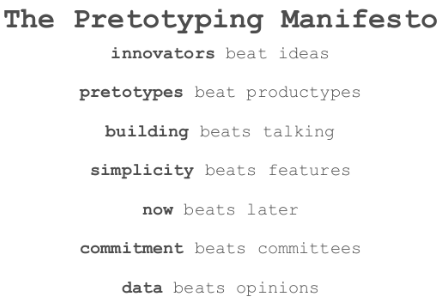
\includegraphics[scale=0.6]{immagini/Manifesto.png}
\end{figure}

\section{Pretotype vs Prototype}
I prototipi aiutano a fallire in fretta, ma spesso non abbastanza in fretta o non abbastanza economicamente.

Più si investe in un'idea e \textbf{più diventa difficile lasciarla morire} e ammettere che era sbagliata, anzi tendenzialmente, una volta ottenuto un buon prototipo che funziona, è facile portarlo avanti investendovi ancora denaro e tempo, pensando che l'aggiunta di funzionalità e features sia la risposta per renderlo vincente.

Molto spesso i prodotti lanciati sul mercato non sono altro che prototipi andati troppo oltre. \textbf{Tra il mondo delle idee astratte e i prototipi funzionanti}, si collocano i \textbf{pretotypes}.

\textbf{Un pretotipo è un semplice mockup del prodotto che si vorrebbe sviluppare} ed è utile per ottenere sia informazioni d'uso che di mercato e, specialmente, per poter prendere decisioni su cosa fare e su cosa non fare.

La \textbf{principale differenza} tra un pretotipo e un prototipo è l'\textbf{investimento}: un \textbf{pretotipo costa molto meno} sia in termini di tempo che in termini di denaro, e consente di fallire in fretta o nel caso, poiché lascia un ampio spazio di manovra, di apportare modifiche.

\pagebreak

\begin{figure}[!h]
	\centering
	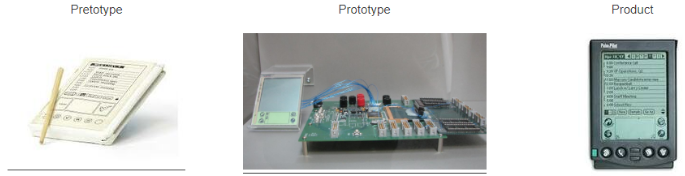
\includegraphics[scale=0.65]{immagini/Pre_prot.png}
\end{figure}

Il \textbf{pretotyping} ha l'obiettivo di aiutare a:

\begin{itemize}
	\item \textbf{Identificare le funzionalità chiave} del nuovo prodotto.
	\item Decidere \textbf{quali} di queste possono o dovrebbero essere \textbf{inserite nel mockup}.
	\item Usare i mockups per il \textbf{test sistematico} e contemporaneamente \textbf{collezionare feedback e dati d'uso}.
	\item Analizzare i dati raccolti per \textbf{determinare il prossimo passo da compiere}.
\end{itemize}

I \textbf{sette pilastri del Pretotyping} sono:

\begin{enumerate}
	\item \textbf{Obbedire alla Legge del Fallimento di Mercato}.
	\item \textbf{Assicurarsi di star costruendo il prodotto giusto}.
	\item \textbf{Non perdersi in chiacchiere, idee o opinioni}.
	\item \textbf{Fidarsi solo dei propri dati, \textbf{TRUST YODA: Your Own DAta}}.
	\item \textbf{Fare pretotyping}.
	\item \textbf{Parlare con i numeri e con i fatti}.
	\item \textbf{Pensare globalmente e non localmente}.
\end{enumerate}

\section{Flusso del Pretotyping}

I \textbf{cinque step} per produrre un buon pretotipo sono i seguenti:

\begin{enumerate}
	\item \textbf{Isolare l'assuzione chiave}: qual è la assunzione o funzionalità chiave dell'idea che, se falsa, ne minerebbe la validità?
	\item \textbf{Scegliere un tipo di pretotype}: quale tipo di pretotyping permette di isolare e testare al meglio le funzionalità chiave?
	\item \textbf{Fare ipotesi di mercato}: quante e quali tipi di persone utilizzeranno il pretotipo? Come lo utilizzeranno? Sarebbe possibile ipotizzare le percentuali di un determinato utilizzo?
	\item \textbf{Testare il pretotype}: mettere il pretotipo nel mondo reale e vedere quante persone sono interessate e quante ci interagiscono. Bisogna partire dal basso, un passo alla volta.
	\item \textbf{Imparare, rifinire, hypozoom}: valutare i risultati, rifinire il pretotipo con i nuovi dati, e se l'ipotesi ha retto, decidere quali altre situazioni testare per ottenere man mano una \textbf{visione completa: hypozooming}.
\end{enumerate}

\pagebreak

\section{Tipi di Pretotyping}
Andiamo ad analizzare alcuni tipi di pretotyping.
\begin{itemize}
	\item Una \textbf{Fake Door} è un marketing entry point per un prodotto che ancora \textbf{non esiste} e può essere utilizzata per \textbf{pubblicizzare} un servizio non ancora pronto e misurare l'interesse degli utenti.

	      È un buon modo per capire se l'oggetto che si vuole sviluppare può avere successo o meno, spendendo pochissimo e quindi, in caso di fallimento, avere un basso impatto economico, inteso sempre sia in termini di denaro che di tempo. Si può usare
	      questo tipo di pretotyping \textbf{quando l'idea può essere descritta in poche e semplici parole}, senza possedere nulla di fisico o materiale.

	      \begin{figure}[!h]
		      \centering
		      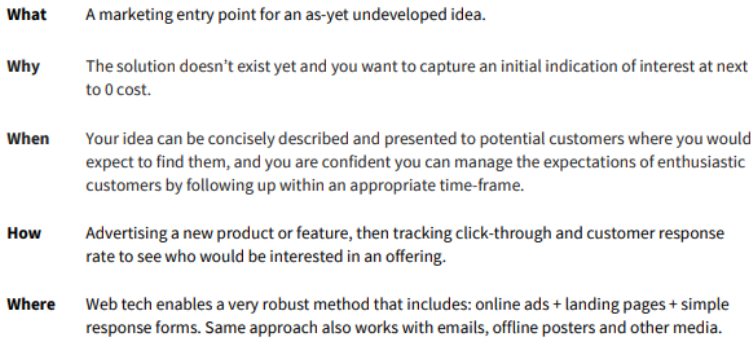
\includegraphics[scale=0.42]{immagini/Fake_door.png}
	      \end{figure}

	\item Si parla di \textbf{Mechanical Turk} quando ci si riferisce ad un oggetto che riesce, nel suo utilizzo, a trasmettere l'esperienza del prodotto finale ad un utente, senza che sia stato sviluppato. Un meachanical turk usa solo man power. È molto utilizzato per sperimentare l'uso e la reale applicabilità di software e algoritmi molto costosi per essere implementati.

	      \begin{figure}[!h]
		      \centering
		      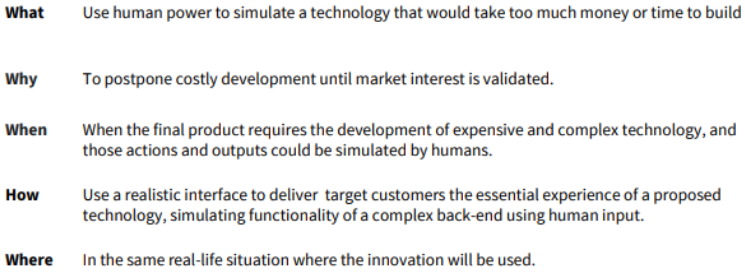
\includegraphics[scale=0.42]{immagini/Mechanical_turk.png}
	      \end{figure}

	\item Un \textbf{Impersonator} è un pretotipo che riesce a far sperimentare un'esperienza realistica all'utente in modo estremamente economico e con un lavoro minimo dietro. Consente cioè di
	      far vivere l'esperienza esattamente come se il prodotto fosse finito e pronto per essere lanciato.

	      \begin{figure}[!h]
		      \centering
		      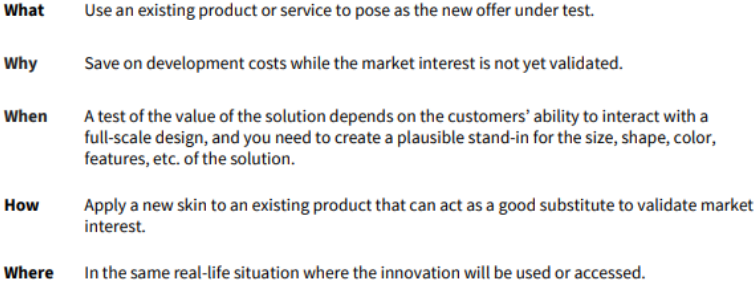
\includegraphics[scale=0.42]{immagini/Impersonator.png}
	      \end{figure}

	      \pagebreak

	\item Un \textbf{Pinocchio} è un pretotipo \textbf{chiaramente falso}, serve per veicolare un messaggio così distante dalla realtà attuale che è faticoso e difficile da spiegare in altri linguaggi naturali. È usato molto spesso per testare l'interesse e il possibile uso di prodotti innovativi e non ancora lanciati da nessuno, nemmeno in maniera simile, sul mercato.

	      \begin{figure}[!h]
		      \centering
		      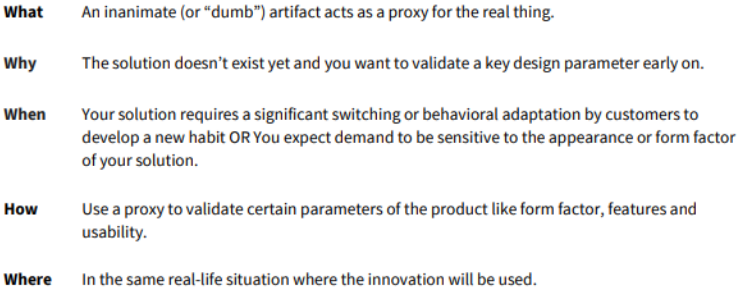
\includegraphics[scale=0.5]{immagini/Pinocchio.png}
	      \end{figure}

	\item Con \textbf{One Night Stand} si indica una \textbf{tecnica di veicolazione} di un pretotipo. Consiste di un \textbf{market test}.
	      Viene usato insieme ad un'altra tecnicha di pretotyping per veicolare meglio il messaggio a una certa cerchia di persone.

	      \begin{figure}[!h]
		      \centering
		      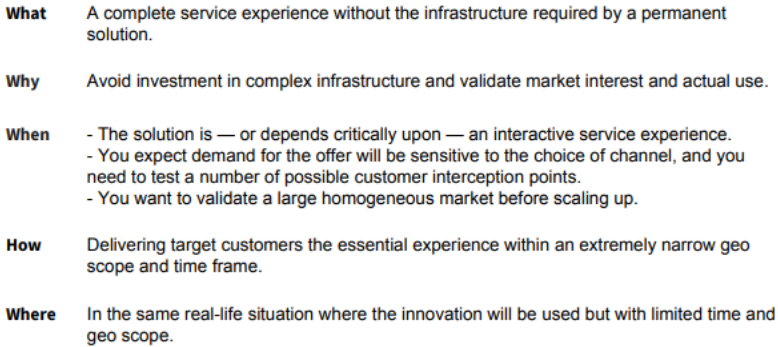
\includegraphics[scale=0.5]{immagini/One_night_stand.png}
	      \end{figure}


	\item Un \textbf{Facade} è una sorta di Impersonator ma è usato per dare un'immagine dell'azienda e non del prodotto stesso. Viene sfruttato spesso per promuovere servizi.

	      \begin{figure}[!h]
		      \centering
		      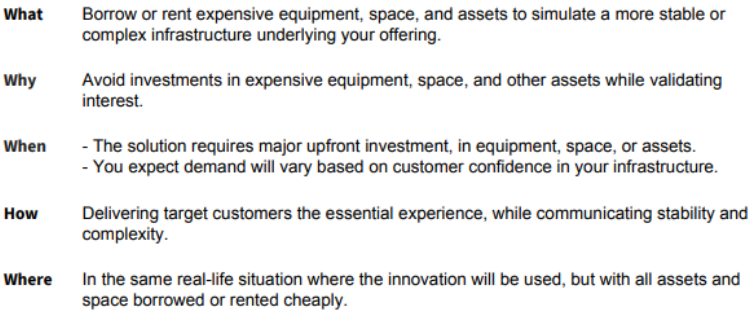
\includegraphics[scale=0.5]{immagini/Facade.png}
	      \end{figure}

\end{itemize}

\pagebreak

\section{Minimum Viable Product}

Dopo varie fasi di pretotyping e aver accumulato sicurezze sufficienti circa il successo del prodotto, lo step successivo è produrre il \textbf{Minimum Viable Product}, cioè la \textbf{versione minimale del prodotto contenente solo ed esclusivamente le features che si sono pretotipate attraverso la fase precedente}.
Non si ha ancora per le mani un prodotto definitivo besì un qualcosa di \textbf{vendibile}, in modo da ottenere del ricavo e dell'utile, che se sufficiente, permetterebbe la produzione definitiva del prodotto.

\begin{figure}[!h]
	\centering
	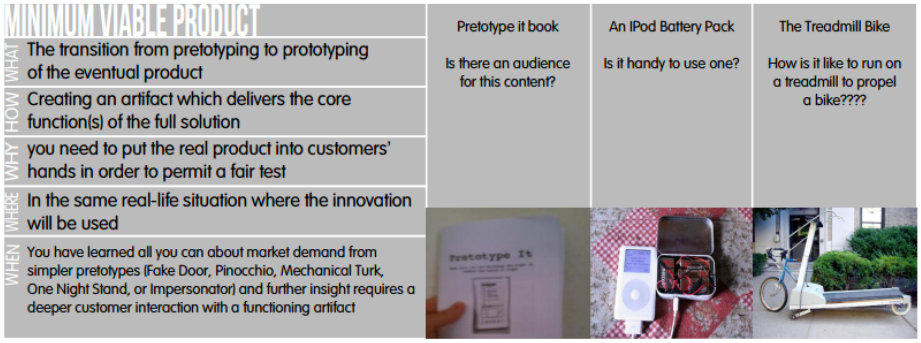
\includegraphics[scale=0.5]{immagini/MVP.png}
	\caption{Minimum Viable Product.}
	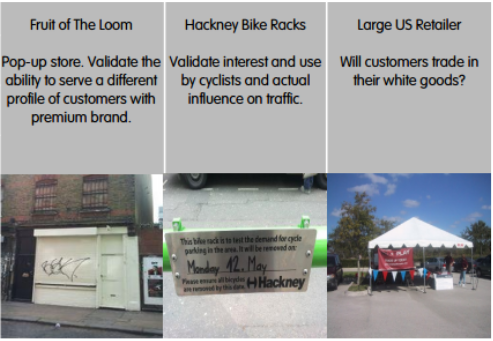
\includegraphics[scale=0.4]{immagini/ONS.png}
	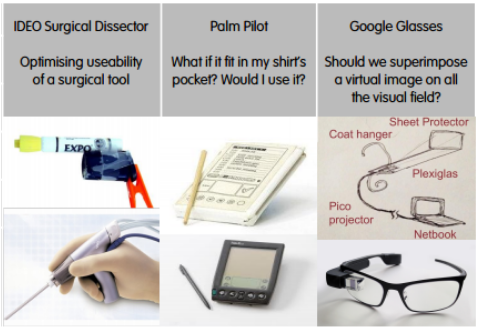
\includegraphics[scale=0.4]{immagini/Pnocc.png}
	\caption{A sinistra esempi di one night stands e a destra esempi di pinocchio.}
	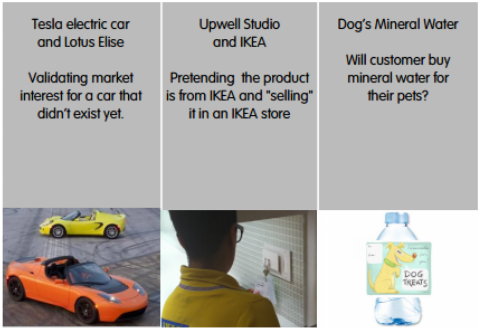
\includegraphics[scale=0.6]{immagini/Imp.png}
	\caption{Esempi di Impersonator.}
\end{figure}

\pagebreak

\chapter{UX for connected devices}

Quando ci si trova di fronte al compito di progettare l'interfaccia di un \textbf{dispositivo
	connesso}, si tende si tende ad adottare un approccio in linea alla \textit{vecchia
	scuola} della UI e UX. Si tende quindi a dare maggior peso e a spendere maggior concentrazione su aspetti come l'estetica delle interfacce e la forma del prodotto fisico. \textbf{Per l'IoT ciò non basta}.

Un prodotto interconnesso può avere un'ottima UI ma una pessima UX, esso non è costituito solamente dalla sua apparenza o dalla sua interfaccia, ma è \textbf{l'insieme delle due cose}.

Internet è un \textbf{mezzo di comunicazione}, fatto dagli uomini per gli uomini, \textbf{l'Internet of Things o IoT è un sistema di dispositivi informatici interconnessi}, macchine meccaniche o digitali \textbf{fornite di un identificatore unico detto UID}.

Esse possiedono la capacità di trasferire i dati sulla rete senza richiedere l'interazione uomo-uomo o uomo-computer.
La differenza tra i due mondi è sottile e spesso gli oggetti IoT sono creati per comunicare perfettamente tra di loro, ma hanno una pessima UI per l'uso umano, e
di conseguenza sono portatori di una pessima UX.

\section{Industry 4.0}

Il termine \textbf{Industria 4.0} indica l'ultima fase del processo con cui l'automazione industriale \textbf{integra} nuove \textbf{tecnologie produttive} per \textbf{migliorare} le condizioni di lavoro, creare nuovi modelli di business e aumentare la produttività e la qualità produttiva degli impianti.

I sistemi computerizzati monitorano i processi fisici, creando copie virtuali del mondo su cui sono basate le scelte e le decisioni future per il business dell'azienda.

\begin{figure}[!h]
	\centering
	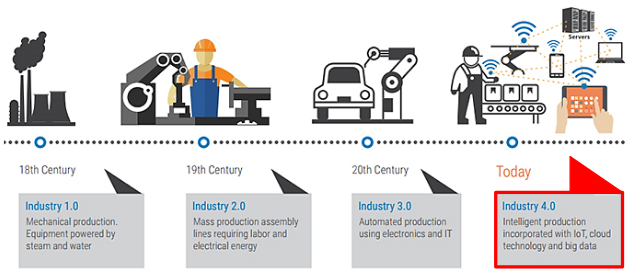
\includegraphics[scale=0.7]{immagini/Industry4.png}
\end{figure}

\pagebreak

Il problema di ogni tappa della rivoluzione industriale risiede nell'aumento esponenziale della \textbf{complessità informatica}. I dati parlano chiaro: il salto informativo dall'industria 3.0 all'industria 4.0 è pari al totale del salto effettuato da quando si usava l'asino come mezzo di locomozione fino alle attuali tecnologie.

\begin{figure}[!h]
	\centering
	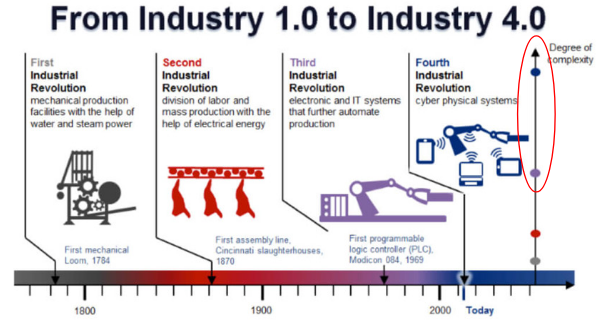
\includegraphics[scale=0.6]{immagini/Revolution.png}
\end{figure}

Quello che prima era un \textbf{processo produttivo}, con l'industria 4.0 diventa un \textbf{servizio} e la quantità di informazione necessaria cresce incredibilmente, di conseguenza progettare per la UX diventa estremamente complesso.

Ma come mai è importante questa evoluzione? Per le seguenti ragioni:

\begin{itemize}
	\item  Ottimizzando la produzione i profitti aumentano.
	\item Sarà possibile creare \textbf{nuovi modelli di business}.
	\item Saranno accessibili \textbf{nuove tecnologie}.
	\item Sarà possibile trasformare la forza lavoro: da operai in tecnici, capaci di estrarre informazioni dalle macchine e modificare la produzione di conseguenza.
\end{itemize}

Il cuore di un sistema interconnesso, sia di tipo consumer che industriale, è il
\textbf{Digital Twin}. Il \textbf{Digital Twin} è  \textbf{una copia digitale di un bene, di una macchina o di un processo reale esistente}. La comunicazione tra l'oggetto fisico e il Digital Twin è \textbf{continua e bidirezionale}. Tale strumento può essere usato sia per logging che per controllo remoto, ma sopratutto, è utile per simulazioni e manutenzione.

\begin{figure}[!h]
	\centering
	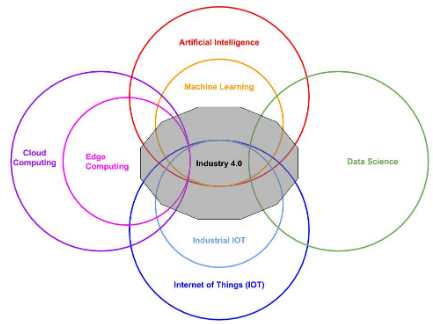
\includegraphics[scale=0.55]{immagini/Holistic.png}
\end{figure}

\pagebreak

\section{Products and Services in the 4.0 era}

\begin{figure}[!h]
	\centering
	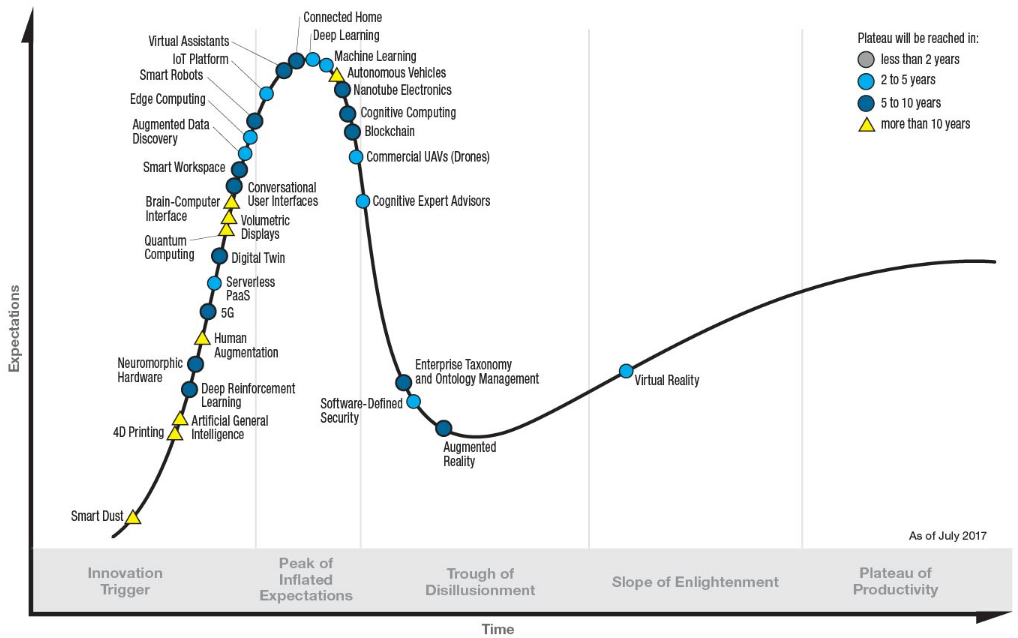
\includegraphics[scale=0.45]{immagini/Hype.png}
	\caption{Gartner Hype Cycle for emerging technologies.}
\end{figure}

L'IoT è solo una tecnologia abilitante, quindi non bisogna progettare per l'IoT bensì bisogna progettare sistemi interconnessi. Ciò altera il paradigma di progettazione: prima erano i computer ad essere dei centri di aggregazione tecnologica: qualche anno fa, ad esempio, in una qualsiasi casa, l'unico oggetto definibile smart era un \textbf{computer}, adesso si hanno più dispositivi connessi per svolgere svariate attività.

Sta sempre più emergendo il concetto di \textbf{intelligenza distribuita} accompagnata da un'\textbf{interfaccia personale}.

I dispositivi che si vuol progettare dovrebbero avere funzionalità altamente \textbf{specifiche} ma veicolate attraverso interfacce \textbf{generiche}. Le interfacce specifiche sono da evitare.

Si prenda, per esempio, un robot da cucina che riesce a fare
di tutto: frullare, centrifugare e cuocere, più una vasta gamma di funzionalità selezionabili, tramite pulsanti, uno per ogni funzione, attraverso un'interfaccia posta sul robot stesso. \textbf{Ciò è da ripudiare} in favore di un robot senza un singolo tasto che capisce da sè cosa va fatto e come farlo.

La progettazione per l'IoT è intrinsecamente più \textbf{complessa} della progettazione di servizi Web. Il design fisico, il design della UX e l'interconnettività di un unico sistema \textbf{non} possono essere gestiti separatamente.

I prodotti connessi pongono i progettisti dinanzi a sfide progettuali nuove, molte delle quali derivano da:

\begin{itemize}
	\item La \textbf{natura} specializzata dei servizi \textbf{IoT}.
	\item La capacità dei dispositivi IoT di fare da \textbf{ponte tra il mondo digitale e fisico}.
	\item Il fatto che molti prodotti IoT siano \textbf{sistemi distribuiti composti da più dispositivi}.
	\item \textbf{Le stranezze del networking}.
\end{itemize}

\pagebreak

\section{Real world context}
Le interfacce, nel mondo dell'IoT, sono sensori e attuatori. I \textbf{sensori} convertono una variabile \textbf{fisica} in un segnale \textbf{elettrico}, mentre gli
attuatori convertono un segnale\textbf{ elettrico} in una variabile \textbf{fisica}.

Gli attuatori possono essere controllati a distanza o automatizzati, ma a differenza dei comandi digitali, le azioni sul mondo reale \textbf{non possono essere annullate}.
Questo contesto fisico di utilizzo crea ulteriori sfide. Nell'IoT non si può dare per
scontato lo stato d'animo dell'utente mentre interagisce con l'oggetto.

Gli oggetti ubiquitari, andando a posizionarsi nei vari angoli della casa o dell'ufficio, si trovano ad interagire con persone che potrebbero momentaneamente \textbf{non essere predisposte all'interazione con un oggetto digitale}, ciò rende l'errore molto più frequente.

Si devono creare quindi oggetti molto semplici sia da capire che da utilizzare.

Un altro aspetto importante è l'\textbf{interusabilità}, cioè la proprietà del sistema di essere usato attraverso \textbf{tutti} i dispositivi o le interfacce che lo compongono (\textit{e.g. Google Assistant può essere usato tramite app, sito web o Google Home}).

\begin{figure}[!h]
	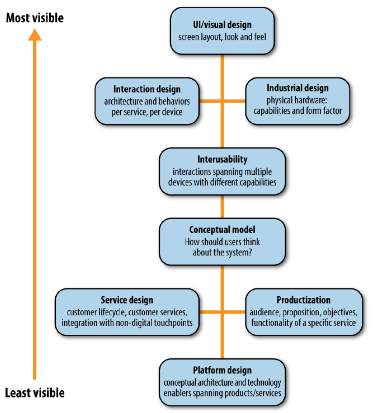
\includegraphics[scale=0.55]{immagini/UX_IoT.png}
	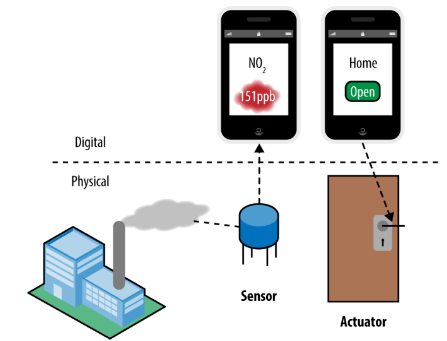
\includegraphics[scale=0.5]{immagini/Sensors_actuators.png}
\end{figure}

\begin{flushleft}
	\textit{Perché puntare così tanto su
		questa caratteristica?}
\end{flushleft}

Bisogna infatti consentire all'utente l'accesso e l'interazione col sistema dove e come egli la desidera, il più compatibilmente possibile con le circostanze in cui egli si trova. L'\textbf{esperienza} dell'utente \textbf{non deve però differire} tra le varie interfacce. Inoltre, gli utenti hanno bisogno di una certa comprensione di come funziona il sistema. Anche i prodotti connessi piuttosto semplici sono concettualmente molto più complessi di quelli non connessi. Quindi è necessario un oggetto che veicoli un modello \textbf{concettuale chiaro}, in modo tale che l'utente si crei un modello mentale solido.

È necessario quindi creare un
\textbf{modello unificato di interazione}, dove è chiaro che l'interfaccia e l'intelligenza sono distribuite, in modo tale da veicolare all'utente un \textbf{unico} modello concettuale utilizzabile per l'intero sistema.

Un'altra problematica è che molti progettisti progettano supponendo che i dispositivi siano sempre connessi, ma questo \textbf{non è sempre vero}! Anzi conviene rovesciare il paradigma, \textbf{progettando per l'assenza di internet e assumendo che sia disponibile solo sporadicamente}. Con questo modo di progettare si considerano anche i ritardi e i problemi dovuti alle reti fisiche e alla trasmissione su di esse.

\chapter{Natural Language}

\begin{figure}[!h]
	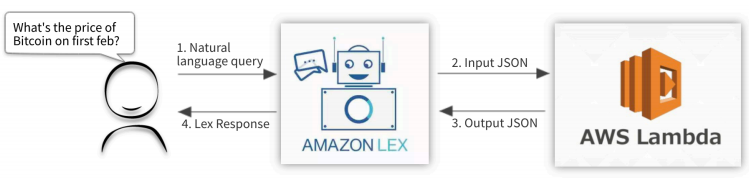
\includegraphics[scale=0.5]{immagini/Natural_language.png}
\end{figure}

Un \textbf{Conversational System} è un'interfaccia uomo macchina in grado di comprendere \textbf{il linguaggio umano} e condurre una conversazione scritta o verbale con l'utente. È un tipo di interfaccia usata per migliorare l'esperienza dell'utente guidandone l'interazione durante l'uso del prodotto.

La conversazione deve essere:
\begin{itemize}
	\item \textbf{Naturale}: l'utente deve poter usare un linguaggio \textbf{spontaneo}, non meccanico o verboso.
	\item \textbf{Accessibile}: l'utente deve capire facilmente e senza nessuna fatica come interagire con l'interfaccia.
	\item \textbf{Efficiente}.
\end{itemize}

Il primo problema che un programmatore deve affrontare quando vuole implementare un'interfaccia del genere è  il seguente: il \textbf{linguaggio naturale è ambiguo}, infatti si possono usare molti costrutti per esprimere il medesimo concetto o impartire il medesimo comando.

Un servizio efficiente per poter scavalcare questo problema è \textbf{Amazon Lex}.

Amazon Lex si basa su due concetti fondamentali: \textbf{speech recognition} e \textbf{natural language understanding}.
Benché esistano molti modi per esprimere il medesimo concetto, un servizio di riconoscimento vocale \textbf{deve essere in grado di capire} ciò che vogliamo fare e quale sia il nostro obiettivo.

Si indicherà con il termine \textbf{intento} l'obbiettivo dell'utente.
Per poter soddisfare l'intento, si deve fare in modo che il sistema riconosca delle \textbf{informazioni chiave} per comprendere il comando. Queste informazioni chiave prendono il nome di \textbf{slots}.

Gli \textbf{slots} sono quindi i dati necessari al conversational system per soddisfare la richiesta dell'utente.

Inoltre per aiutare il sistema ad interagire con gli utenti e a riconoscere il comando si definiscono anche delle \textbf{utterances}, ovvero delle frasi di esempio con diversa struttura ma uguale significato. Un insieme di \textbf{utterances} fa riferimento ad un \textbf{intento}.

Infine si procede a definire la sequenza d'interazione tra l'utente e il conversational system  fornendo a quest ultimo dei \textbf{prompts}, ovvero la risposta che l'interfaccia darà all'utente dopo ogni comando ricevuto.

\pagebreak

\textbf{AWS Lambda} è una piattaforma di calcolo \textbf{event-driven} e \textbf{serverless} che Amazon fornisce come parte dei suoi \textbf{servizi web}: mette in esecuzione del codice in risposta ad eventi e ne gestisce le risorse computazionali.

\begin{figure}[!h]
	\centering
	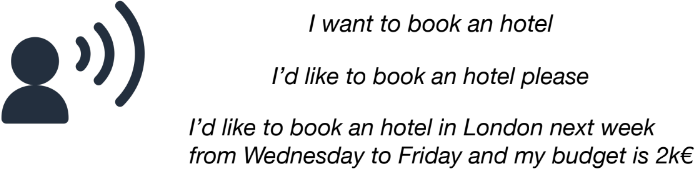
\includegraphics[scale=0.55]{immagini/Lex_general3.png}
	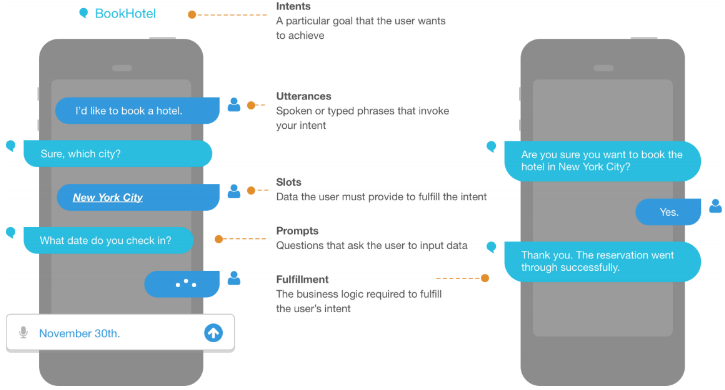
\includegraphics[scale=0.65]{immagini/Lex_general.png}
	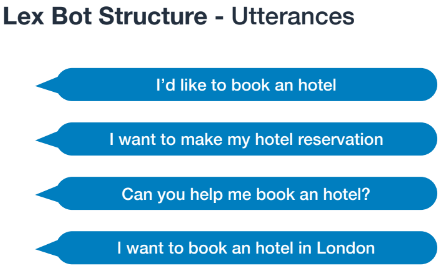
\includegraphics[scale=0.6]{immagini/Lex_general1.png}
	\includegraphics[scale=0.5]{immagini/Lex_general2.png}
\end{figure}
\end{document}